\documentclass[11.5pt,aspectratio=169,handout]{beamer}

\usepackage[utf8]{inputenc}
\usepackage[T1]{fontenc}
\usepackage{lmodern}
\usepackage[spanish,es-lcroman]{babel}
\usepackage{csquotes}
\addto\shorthandsspanish{\spanishdeactivate{~<>}}
\selectlanguage{spanish}
\usepackage{amsmath,amsfonts,amssymb}
\usepackage{graphicx,booktabs}
\usepackage{adjustbox}
\graphicspath{{../Figuras/}}
% Evita "Incompatible glue units" [babel español \% + \, dentro de adjustbox]:
% redefine \% a un porcentaje simple sin el gobble de espacios del español.
\AtBeginDocument{\def\%{\char37\relax}}
\usepackage{xcolor}
\usepackage{ragged2e}
\usepackage{tikz}
\usetikzlibrary{calc,positioning,arrows.meta,shapes.geometric,shapes,matrix,fit}
\usepackage{colortbl,multirow,tabularray}
\usepackage{multicol}
%------------------------------------------------------------------
% COLORES PERSONALIZADOS [paleta del PPTX]
%------------------------------------------------------------------
\definecolor{azulUSACH}{RGB}{0,130,130}
\definecolor{azulBox}{RGB}{68,114,196}
\definecolor{azulBg}{RGB}{210,228,255}
\definecolor{rojoBox}{RGB}{192,80,77}
\definecolor{rojoBg}{RGB}{255,228,220}
\definecolor{violetaBox}{RGB}{112,48,160}
\definecolor{violetaBg}{RGB}{230,215,245}
\definecolor{verdeBox}{RGB}{84,130,53}
\definecolor{verdeBg}{RGB}{210,240,210}
\definecolor{grisBox}{RGB}{140,140,140}
\definecolor{grisBg}{RGB}{230,228,222}
\definecolor{naranjaBox}{RGB}{197,144,0}
\definecolor{naranjaBg}{RGB}{255,245,210}

%------------------------------------------------------------------
% TEMA
%------------------------------------------------------------------
\usetheme{Madrid}
\usecolortheme{dolphin}
\setbeamercovered{transparent}
\setbeamercolor{alerted text}{fg=blue!75!black}
\setbeamercolor{block title}{bg=blue!20}

% Lamina.png: zona blanca inicia en 25.9mm; margen ajustado para coincidir con borde rojo
% textwidth = 160 - 26 - 4 = 130mm
\setbeamersize{text margin left=2.6cm, text margin right=0.4cm}

%------------------------------------------------------------------
% BIBLIOGRAFÍA
%------------------------------------------------------------------
%\usepackage[backend=biber, style=authoryear]{biblatex}
%\addbibresource{biblio.bib}
%\renewcommand*{\bibfont}{\tiny}
%\setlength\bibitemsep{0pt}
%\setlength\bibhang{1em}
%\AtEveryBibitem{\clearfield{url}\clearfield{urldate}}

%------------------------------------------------------------------
% PIE DE PÁGINA [alineado con el borde izquierdo del área roja]
%------------------------------------------------------------------
\setbeamercolor{footline bar}{bg=white,fg=black}
% Tamaño explícito del pie: idéntico en footline normal y en \addplainfoot
\setbeamerfont{author in head/foot}{size={\fontsize{6pt}{7.2pt}\selectfont}}
\setbeamertemplate{footline}{%
  \vspace{5mm}%
  \begin{beamercolorbox}[wd=\paperwidth,ht=2.5ex,dp=1.5ex,%
      leftskip=2.6cm,rightskip=0.4cm]{footline bar}%
    {\color{black}\usebeamerfont{author in head/foot}%
    Examen de Título\hfill\insertshortauthor\hfill%
    \insertframenumber{} / \inserttotalframenumber}%
  \end{beamercolorbox}%
}
\setbeamertemplate{navigation symbols}{}
\setbeamertemplate{caption}[numbered]
\setbeamerfont{caption}{size=\scriptsize}

%------------------------------------------------------------------
% FRAMETITLE: centrado en la zona roja de referencia
%------------------------------------------------------------------
\setbeamertemplate{frametitle}{%
  \nointerlineskip%
  \begin{beamercolorbox}[wd=\paperwidth,sep=0.3cm]{frametitle}%
    \usebeamerfont{frametitle}%
    \hspace{2.3cm}%
    \makebox[\dimexpr\paperwidth-2.6cm-0.4cm\relax][c]{%
      \underline{\insertframetitle}%
    }%
  \end{beamercolorbox}%
}
\newcommand{\ctitle}[1]{\frametitle{#1}}

%==================================================================
% SISTEMA DE DISEÑO [minimalista, formato único]
% Cambiar un valor aquí re-estiliza todo el documento.
%==================================================================
% Tamaños base
\newcommand{\tablasize}{\scriptsize}      % único tamaño para tablas de datos
\newcommand{\capsize}{\scriptsize}        % captions de figuras/tablas
\renewcommand{\arraystretch}{1.1}         % alto de fila uniforme

% Espaciados permitidos [usar SOLO estos]
\newcommand{\gA}{\vspace{1mm}}            % gap chico
\newcommand{\gB}{\vspace{2mm}}            % gap medio [entre bloques]
\newcommand{\gC}{\vspace{3.5mm}}          % gap grande [separar secciones]

% Alturas estándar de imagen [minimalista: 3 tamaños fijos]
\newcommand{\imghS}{2.4cm}                % imágenes apiladas [par en columna]
\newcommand{\imghM}{4.2cm}                % imagen principal en 2 columnas
\newcommand{\imghL}{5.6cm}                % imagen única a ancho de slide

% Subtítulo de sección [azulUSACH, negrita, espaciado fijo]
\newcommand{\subtitulo}[1]{%
  \vspace{-3mm}\begin{center}\textcolor{azulUSACH}{\textbf{#1}}\end{center}\gA}

% Título + subtítulo combinados [frames "RESULTADOS Y COMPARATIVAS"]
\newcommand{\ctitlesub}[2]{\ctitle{#1}\subtitulo{#2}}

% Caption de figura unificado: \figcap{N}{descripción}{fuente}
\newcommand{\figcap}[3]{{\capsize Figura #1: #2.\\ Fuente: #3.}}

% Wrapper de imagen estándar [ancho completo]: \fig{altura}{archivo}
\newcommand{\fig}[2]{\includegraphics[width=\linewidth,height=#1,keepaspectratio]{#2}}

% Wrapper de tabla: mantiene \tablasize si cabe; reduce solo si excede \linewidth
% [preserva toda la info, nunca agranda]. Uso: \fittab{\tablasize\begin{tabular}...}
\newcommand{\fittab}[1]{\adjustbox{max width=\linewidth}{#1}}
%==================================================================

% Pie de página para frames [plain] [portada, TOC, contraportada]
\newcommand{\addplainfoot}{%
  \begin{tikzpicture}[remember picture,overlay]
    % font pequeño antes de la caja: ex (ht/dp) se calcula al tamaño del pie;
    % xshift=2.6cm compensa el overhang del leftskip para alinear con x=0
    \node[anchor=south west,inner sep=0] at ([xshift=2.6cm]current page.south west){%
      \usebeamerfont{author in head/foot}%
      \begin{beamercolorbox}[wd=\paperwidth,ht=2.5ex,dp=1.5ex,%
          leftskip=2.6cm,rightskip=0.4cm]{footline bar}%
        {\color{black}\usebeamerfont{author in head/foot}%
        Examen de Título\hfill\insertshortauthor\hfill%
        \insertframenumber{} / \inserttotalframenumber}%
      \end{beamercolorbox}};
  \end{tikzpicture}%
}

%------------------------------------------------------------------
% DATOS DEL DOCUMENTO
%------------------------------------------------------------------
\title{{\large Comparación del diseño estructural de un galpón de acero en base
        a la actualización de la norma sísmica [NCh2369]\\
        y la norma de viento~\mbox{[NCh432]}}}

\subtitle{{\small \vspace{3mm} Examen de Título — Para optar al Título de Ingeniero
Civil en Obras Civiles}}

\author[B. Franco, C. Bordones]{%
  {\small \textbf{Bruno Alonso Franco Sentis} \quad \textbf{Cristofer Walter Bordones Armijo}}\\[5mm]
  {\footnotesize Profesor Guía: Jorge Pi Luco\\
   Comisión: Luis Leiva Aravena, Fernando Ibáñez Lara\\
   Departamento de Ingeniería en Obras Civiles}}

\date{{\footnotesize 30 de Junio de 2026}}

%==================================================================
\begin{document}
%==================================================================

\usebackgroundtemplate{%
  
\includegraphics[width=\paperwidth,height=0.96\paperheight]{Lamina.png}}

%------------------------------------------------------------------
% 1. PORTADA
%------------------------------------------------------------------
\begin{frame}[plain]
  \vspace*{0.5cm}
  \titlepage
  \addplainfoot
\end{frame}

%------------------------------------------------------------------
% 2. TABLA DE CONTENIDOS
%------------------------------------------------------------------
\begin{frame}[plain]
  \ctitle{TABLA DE CONTENIDOS}
  \begin{multicols}{2}
    \tableofcontents
  \end{multicols}
  \addplainfoot
\end{frame}


%==================================================================
\section{Resumen Presentación N°1}
%==================================================================

%------------------------------------------------------------------
% 3. RESUMEN N°1: EL PROYECTO Y EL PROBLEMA
%------------------------------------------------------------------
\begin{frame}
\ctitle{RESUMEN N°1: EL PROYECTO Y EL PROBLEMA}
\begin{columns}[T,totalwidth=\textwidth]
  \column{0.55\textwidth}
  \vspace{-1mm}
  \begin{itemize}\footnotesize\setlength{\itemsep}{3mm}
    \item Caso de estudio: \alert{Nave~F}, galpón industrial
          de acero [Metalpar, Maipú], recepcionado el
          año 2025.
    \item Diseñado con normas \alert{oficiales}:
          \alert{NCh2369.Of2003} [sismo] y \alert{NCh432.Of1971}
          [viento].
    \item La actualización de estas normativas en 2025 hace
          imperativa una \alert{reevaluación estructural} bajo
          los nuevos parámetros.
    \item \textbf{Problema:} Determinación de la variación en
          las solicitaciones de diseño y la \alert{carga gobernante}
          tras la aplicación de las normativas de 2025.
  \end{itemize}
  \column{0.42\textwidth}
  \vfill
  \centering
  \includegraphics[width=\linewidth,height=\imghM,keepaspectratio]%
    {slide03_fig01.png}\\[1mm]
  \figcap{1}{Galpón industrial de acero [tipología de estudio]}{Modelo IFC maestranza}
  \vfill
\end{columns}
\end{frame}

%------------------------------------------------------------------
% 4. RESUMEN N°1: OBJETIVOS E HIPÓTESIS
%------------------------------------------------------------------
\begin{frame}
\ctitle{RESUMEN N°1: OBJETIVOS E HIPÓTESIS}
\vspace{-1mm}
{\footnotesize\textbf{Objetivo general:} comparar la respuesta estructural de la Nave~F ante sismo y viento
bajo el marco normativo original y sus actualizaciones 2025 [cortes basales,
desplazamientos, F.U. y solicitaciones].}

\vspace{2mm}
{\footnotesize\textbf{Objetivos específicos:}}\\[1mm]
\begin{columns}[T,totalwidth=\textwidth]
  \column{0.52\textwidth}
  \begin{itemize}\footnotesize\setlength{\itemsep}{1.5mm}
    \item \alert{Levantar} la estructura [geometría, perfiles,
          sistema].
    \item \alert{Determinar} acciones de sismo y viento en
          ambos marcos.
    \item \alert{Modelar} en SAP2000 y obtener la respuesta
          global.
    \item \alert{Verificar} elementos principales.
    \item \alert{Proponer} adecuación conceptual donde no
          cumpla.
  \end{itemize}
  \column{0.45\textwidth}
  \vspace{2mm}
  \begin{beamercolorbox}[rounded=true,shadow=true,sep=3mm]{block body}
  {\footnotesize\textbf{Hipótesis}}\\[1mm]
  {\footnotesize La \alert{NCh432:2025} [viento] \alert{reduce} las presiones
  para este sitio; la \alert{NCh2369:2025} [sismo]
  \alert{aumenta} las solicitaciones. Se presume un
  \alert{cambio de la carga dominante}: de viento a
  sismo.}
  \end{beamercolorbox}
\end{columns}
\end{frame}

%------------------------------------------------------------------
% 5. RESUMEN N°1: ALCANCES, LIMITACIONES Y MÉTODO
%------------------------------------------------------------------
\begin{frame}
\ctitle{RESUMEN N°1: ALCANCES, LIMITACIONES Y MÉTODO}
\vspace{2mm}
\begin{columns}[T,totalwidth=\textwidth]
  \column{0.48\textwidth}
  {\footnotesize\textbf{Alcances:}}
  \begin{itemize}\footnotesize\setlength{\itemsep}{1.5mm}
    \item Acero \alert{A270~ES} [principales y secundarios].
    \item Diseño \alert{AISC~360-10} / \alert{NCh427/1}.
    \item Sismo \alert{NCh2369} Oficial 2003 y 2025.
    \item Viento \alert{NCh432} Oficial 1971 y 2025.
    \item Verificación de \alert{elementos principales}.
  \end{itemize}
  \column{0.48\textwidth}
  {\footnotesize\textbf{Limitaciones:}}
  \begin{itemize}\footnotesize\setlength{\itemsep}{1.5mm}
    \item Análisis de \alert{costo} por kilogramo de acero.
    \item Refuerzos a nivel \alert{conceptual}.
    \item Materiales según \alert{especificaciones técnicas}.
    \item \alert{SAP2000} v24.2.0.
  \end{itemize}
\end{columns}
\vspace{3mm}
{\footnotesize El \textbf{método} de trabajo [levantamiento $\to$ análisis normativo $\to$ modelación $\to$ comparación] se
detalla a continuación.}
\end{frame}


%==================================================================
\section{Metodología}
%==================================================================

%------------------------------------------------------------------
% 6. METODOLOGÍA
%------------------------------------------------------------------
\begin{frame}
\ctitle{METODOLOGÍA}
\vspace{2mm}
\begin{center}
  \includegraphics[height=0.78\textheight,keepaspectratio]%
    {diapo6.png}
\end{center}
\end{frame}

%------------------------------------------------------------------
% 7. METODOLOGÍA [2]
%------------------------------------------------------------------
\begin{frame}
\ctitle{METODOLOGÍA}
\vspace{2mm}
\begin{center}
  \includegraphics[height=0.78\textheight,keepaspectratio]%
    {metodologia.png}
\end{center}
\end{frame}

%------------------------------------------------------------------
% 7b. METODOLOGÍA — ETAPA 1: Recopilación de antecedentes
%------------------------------------------------------------------
\begin{frame}
\ctitle{METODOLOGÍA}
\vspace{1mm}
\begin{center}
{\large\bfseries ETAPA 1}\\[1mm]
{\small Recopilación de antecedentes}
\end{center}
\vspace{2mm}
\begin{center}
\begin{tikzpicture}
  % Dashed surrounding box
  \draw[dashed, rounded corners=6pt, grisBox, thick]
    (0,0) rectangle (10.8,3.2);
  \node[anchor=north east, font=\tiny\itshape, grisBox] at (10.8,3.2)
    {Simultáneo};
  % Left box
  \filldraw[draw=azulBox!80!black, fill=azulBg, rounded corners=4pt]
    (0.2,0.2) rectangle (5.0,3.0);
  \node[font=\small\bfseries, azulBox!80!black] at (2.6,2.35)
    {Investigación normativa};
  \node[font=\scriptsize, align=center] at (2.6,1.35)
    {NCh2369 y NCh432\\(versiones oficial y 2025)};
  % Bidirectional arrow
  \draw[<->, thick, grisBox!80] (5.15,1.6)--(5.65,1.6);
  % Right box
  \filldraw[draw=verdeBox!80!black, fill=verdeBg, rounded corners=4pt]
    (5.8,0.2) rectangle (10.6,3.0);
  \node[font=\small\bfseries, verdeBox!80!black] at (8.2,2.35)
    {Levantamiento en terreno};
  \node[font=\scriptsize, align=center] at (8.2,1.35)
    {Geometría, perfiles,\\conexiones, materialidad};
\end{tikzpicture}
\end{center}
\end{frame}

%------------------------------------------------------------------
% 7c. METODOLOGÍA — ETAPA 2: Análisis normativo
%------------------------------------------------------------------
\begin{frame}
\ctitle{METODOLOGÍA}
\vspace{1mm}
\begin{center}
{\large\bfseries ETAPA 2}\\[1mm]
{\small Análisis normativo}
\end{center}
\vspace{2mm}
\begin{center}
\begin{tikzpicture}
  \draw[dashed, rounded corners=6pt, grisBox, thick]
    (0,0) rectangle (10.8,3.2);
  \node[anchor=north east, font=\tiny\itshape, grisBox] at (10.8,3.2)
    {Simultáneo};
  % Left box (NCh432 - rojo/naranja)
  \filldraw[draw=rojoBox!80!black, fill=rojoBg, rounded corners=4pt]
    (0.2,0.2) rectangle (5.0,3.0);
  \node[font=\small\bfseries, rojoBox!80!black] at (2.6,2.35)
    {Análisis NCh432};
  \node[font=\scriptsize, align=center] at (2.6,1.35)
    {Cargas de viento\\Versión oficial vs 2025};
  % Bidirectional arrow
  \draw[<->, thick, grisBox!80] (5.15,1.6)--(5.65,1.6);
  % Right box (NCh2369 - naranja/beige)
  \filldraw[draw=naranjaBox!80!black, fill=naranjaBg, rounded corners=4pt]
    (5.8,0.2) rectangle (10.6,3.0);
  \node[font=\small\bfseries, naranjaBox!80!black] at (8.2,2.35)
    {Análisis NCh2369};
  \node[font=\scriptsize, align=center] at (8.2,1.35)
    {Cargas sísmicas\\Versión oficial vs 2025};
\end{tikzpicture}
\end{center}
\end{frame}

%------------------------------------------------------------------
% 7d. METODOLOGÍA — ETAPA 3: Modelación estructural
%------------------------------------------------------------------
\begin{frame}
\ctitle{METODOLOGÍA}
\vspace{1mm}
\begin{center}
{\large\bfseries ETAPA 3}\\[1mm]
{\small Modelación estructural}
\end{center}
\vspace{2mm}
\begin{center}
\begin{tikzpicture}
  \draw[dashed, rounded corners=6pt, grisBox, thick]
    (0,0) rectangle (10.8,3.2);
  \node[anchor=north east, font=\tiny\itshape, grisBox] at (10.8,3.2)
    {Simultáneo};
  % Left box
  \filldraw[draw=violetaBox!70!black, fill=violetaBg, rounded corners=4pt]
    (0.2,0.2) rectangle (5.0,3.0);
  \node[font=\small\bfseries, violetaBox!80!black] at (2.6,2.35)
    {Modelo SAP2000};
  \node[font=\scriptsize, align=center] at (2.6,1.35)
    {Galpón con\\normativa oficial};
  % Bidirectional arrow
  \draw[<->, thick, grisBox!80] (5.15,1.6)--(5.65,1.6);
  % Right box
  \filldraw[draw=violetaBox!70!black, fill=violetaBg, rounded corners=4pt]
    (5.8,0.2) rectangle (10.6,3.0);
  \node[font=\small\bfseries, violetaBox!80!black] at (8.2,2.35)
    {Modelo SAP2000};
  \node[font=\scriptsize, align=center] at (8.2,1.35)
    {Galpón con normativa\\actualizada 2025};
\end{tikzpicture}
\end{center}
\end{frame}

%------------------------------------------------------------------
% 7e. METODOLOGÍA — ETAPA 4: Comparación de resultados
%------------------------------------------------------------------
\begin{frame}
\ctitle{METODOLOGÍA}
\vspace{1mm}
\begin{center}
{\large\bfseries ETAPA 4}\\[1mm]
{\small Comparación de resultados}
\end{center}
\vspace{1mm}
\begin{center}
\begin{tikzpicture}[node distance=0.3cm]
  % Top box
  \filldraw[draw=verdeBox!80!black, fill=verdeBg, rounded corners=5pt]
    (0.2,3.2) rectangle (10.6,4.2);
  \node[font=\small\bfseries, verdeBox!80!black] at (5.4,3.7)
    {Análisis comparativo de la respuesta estructural};
  % Arrows down
  \foreach \x in {1.8, 5.4, 9.0}
    \draw[-Stealth, thick, grisBox!80] (\x,3.2)--(\x,2.85);
  % Three boxes below
  \filldraw[draw=rojoBox!70!black, fill=rojoBg, rounded corners=4pt]
    (0.2,0.1) rectangle (3.4,2.8);
  \node[font=\scriptsize\bfseries, rojoBox!80!black, align=center] at (1.8,2.25)
    {Cortes\\basales};
  \node[font=\tiny, align=center] at (1.8,1.3) {Variación por\\norma};

  \filldraw[draw=naranjaBox!70!black, fill=naranjaBg, rounded corners=4pt]
    (3.8,0.1) rectangle (7.0,2.8);
  \node[font=\scriptsize\bfseries, naranjaBox!80!black, align=center] at (5.4,2.25)
    {Desplaza-\\mientos máx.};
  \node[font=\tiny, align=center] at (5.4,1.3) {Derivas de\\entrepiso};

  \filldraw[draw=verdeBox!70!black, fill=verdeBg, rounded corners=4pt]
    (7.4,0.1) rectangle (10.6,2.8);
  \node[font=\scriptsize\bfseries, verdeBox!80!black, align=center] at (9.0,2.25)
    {Factores de\\utilización};
  \node[font=\tiny, align=center] at (9.0,1.3) {Capacidad vs\\demanda};
\end{tikzpicture}
\end{center}
\end{frame}

%------------------------------------------------------------------
% 7f. METODOLOGÍA — ETAPA 5: Cierre
%------------------------------------------------------------------
\begin{frame}
\ctitle{METODOLOGÍA}
\vspace{-10mm}
\begin{center}
{\large\bfseries ETAPA 5}\\[1mm]
{\small Cierre}
\end{center}
\vspace{2mm}
\begin{center}
\begin{tikzpicture}
  \filldraw[draw=grisBox!70!black, fill=grisBg, rounded corners=8pt]
    (0,0) rectangle (10.8,1.5);
  \node[font=\normalsize\bfseries, grisBox!80!black] at (5.4,0.75)
    {Conclusiones y recomendaciones};
\end{tikzpicture}
\end{center}
\end{frame}


%==================================================================
\section{Recopilación de antecedentes}
%==================================================================

%------------------------------------------------------------------
% 8. RECOPILACIÓN DE ANTECEDENTES
%------------------------------------------------------------------
\begin{frame}
\ctitle{RECOPILACIÓN DE ANTECEDENTES}
\begin{columns}[T,totalwidth=\textwidth]
  \column{0.50\textwidth}
  \vspace{-1mm}
  \begin{itemize}\footnotesize\setlength{\itemsep}{2.5mm}
    \item \textbf{Punto de partida:} planos estructurales y
          \alert{memoria de cálculo original} [PLG
          Ingenieros, 2023].
    \item Corroboración de la geometría con planos de fabricación
          [maestranza].
    \item Normas del diseño original:
          \alert{NCh2369.Of2003} [sismo], \alert{NCh432.Of1971}
          [viento], NCh3171 2010, NCh1537 2009, NCh431 1977.
    \item Materialidad original: \alert{A270 ES}; pernos de unión A325,
          secundarios A307, anclaje A36.
    \item Estos antecedentes se \alert{replican} para
          construir el modelo de la condición
          instalada.
  \end{itemize}
  \column{0.47\textwidth}
  \vfill
  \centering
  \includegraphics[width=\linewidth,height=\imghM,keepaspectratio]%
    {slide12_fig02.png}\\[1mm]
  \figcap{2}{Elevaciones planos de maestranza}{Planos maestranza}
  \vfill
\end{columns}
\end{frame}

%------------------------------------------------------------------
% 8b. RECOPILACIÓN — FIGURA 2 A PÁGINA COMPLETA
%------------------------------------------------------------------
\begin{frame}
\ctitle{RECOPILACIÓN DE ANTECEDENTES}
\vspace{1mm}
\begin{center}
  \includegraphics[width=\linewidth,height=0.80\textheight,keepaspectratio]%
    {slide12_fig02.png}\\[1mm]
  \figcap{2}{Elevaciones planos de maestranza}{Planos maestranza}
\end{center}
\end{frame}


%==================================================================
\section{Descripción de la Nave F}
%==================================================================

%------------------------------------------------------------------
% 9. DESCRIPCIÓN: UBICACIÓN Y ANTECEDENTES
%------------------------------------------------------------------
\begin{frame}
\ctitle{DESCRIPCIÓN: UBICACIÓN Y ANTECEDENTES}
\begin{columns}[T,totalwidth=\textwidth]
  \column{0.45\textwidth}
  \vspace{-1mm}
  \begin{itemize}\footnotesize\setlength{\itemsep}{2.5mm}
    \item Propietario: \alert{Metalpar}.
    \item Ubicación: Camino Melipilla
          N°9236, \alert{Maipú} [R.M.].
    \item Año de recepción: \alert{2025}.
    \item Galpón industrial de acero, planta
          rectangular \alert{$50 \times 83{,}5$~m} [$\approx$\alert{4.175
          m$^2$}].
    \item \alert{10 marcos} transversales; luz
          transversal de \alert{50~m}.
  \end{itemize}
  \column{0.52\textwidth}
  \vfill
  \centering
  \includegraphics[width=\linewidth,height=\imghS,keepaspectratio]%
    {slide13_fig03.png}\\[1mm]
  \figcap{3}{Vista general de la Nave~F}{Elaboración propia}\\[2mm]
  \includegraphics[width=0.7\linewidth,height=2.0cm,keepaspectratio]%
    {slide13_fig04.png}\\[1mm]
  \figcap{4}{Ubicación [Maipú]}{Elaboración propia}
  \vfill
\end{columns}
\end{frame}

%------------------------------------------------------------------
% 10. GEOMETRÍA: PLANTA Y ELEVACIÓN
%------------------------------------------------------------------
\begin{frame}
\ctitle{GEOMETRÍA: PLANTA DE EJES}
\vspace{-4mm}
\begin{center}
  \includegraphics[width=0.95\textwidth,height=0.74\textheight,keepaspectratio]%
    {slide14_fig05.png.png}\\[2mm]
  \figcap{5}{Planta de ejes --- 10 marcos, separación 10~m [1.\textsuperscript{er} vano 6,5~m; último 7~m]}{Elaboración propia}
\end{center}
\end{frame}

%------------------------------------------------------------------
% 10b. GEOMETRÍA: ELEVACIÓN TRANSVERSAL
%------------------------------------------------------------------
\begin{frame}
\ctitle{GEOMETRÍA: ELEVACIÓN TRANSVERSAL}
\vspace{2mm}
\begin{center}
  \includegraphics[width=0.95\textwidth,height=0.78\textheight,keepaspectratio]%
    {slide14_fig06.png}\\[2mm]
  \figcap{6}{Elevación transversal tipo --- hombro 7,53~m, cumbrera 8,85~m; dos aguas [$\theta \approx 3{,}02^\circ$]}{Elaboración propia}
\end{center}
\end{frame}


%==================================================================
\section{Levantamiento en terreno}
%==================================================================

%------------------------------------------------------------------
% 11. LEVANTAMIENTO EN TERRENO
%------------------------------------------------------------------
\begin{frame}
\ctitle{LEVANTAMIENTO EN TERRENO}
\begin{columns}[T,totalwidth=\textwidth]
  \column{0.48\textwidth}
  \vspace{-1mm}
  \begin{itemize}\footnotesize\setlength{\itemsep}{2.5mm}
    \item Visita a terreno: \alert{11 de enero de
          2026}. Inspección visual, medición
          directa y registro fotográfico
          sistemático.
    \item Cotas: huincha métrica y \alert{medición
          láser}.
    \item Espesores en secciones cerradas:
          \alert{medidor ultrasónico} [pulso-eco];
          espesores visibles con pie de metro
          digital.
    \item Producto: \alert{Modelo SAP2000} que
          reproduce la condición instalada.
  \end{itemize}
  \column{0.49\textwidth}
  \vfill
  \centering
  \includegraphics[width=\linewidth,height=\imghM,keepaspectratio]%
    {slide15_fig08.png}\\[1mm]
  \figcap{7}{Registro fotográfico - riostras y pilares}{Elaboración propia}
  \vfill
\end{columns}
\end{frame}


%==================================================================
\section{Discrepancia planos vs construido}
%==================================================================

%------------------------------------------------------------------
% 12. DISCREPANCIA: PLANOS VS CONSTRUIDO
%------------------------------------------------------------------
\begin{frame}
\ctitle{DISCREPANCIA: PLANOS VS CONSTRUIDO}
\vspace{2mm}
{\footnotesize El contraste planos vs condición construida arrojó \alert{dos hallazgos}
[en \textcolor{red}{rojo}, lo que difiere del proyecto]:}
\vspace{3mm}
\begin{itemize}\small\setlength{\itemsep}{4mm}
  \item Pilares secundarios [ejes 1 y 10]: proyectados J2 $\to$ ejecutados
        como \alert{P2} [{[}\,{]} $150\times150\times3$].
  \item Vigas longitudinales: \alert{PT1} solo en ejes 2-3 y 8-9; el resto, \alert{PT2}.
  \item Ambas diferencias se \alert{incorporan al modelo} [representa la estructura
        realmente instalada].
\end{itemize}
\end{frame}

%------------------------------------------------------------------
% 12b. DISCREPANCIA: PLANTA CONSTRUIDA [Figura 8]
%------------------------------------------------------------------
\begin{frame}
\ctitle{DISCREPANCIA: PLANTA CONSTRUIDA}
\vspace{2mm}
\begin{center}
  \includegraphics[width=0.95\textwidth,height=0.74\textheight,keepaspectratio]%
    {slide16_fig09.png}\\[2mm]
  \figcap{8}{Planta construida [P2 en rojo]}{Elaboración propia}
\end{center}
\end{frame}

%------------------------------------------------------------------
% 12c. DISCREPANCIA: ELEVACIÓN CONSTRUIDA [Figura 9]
%------------------------------------------------------------------
\begin{frame}
\ctitle{DISCREPANCIA: ELEVACIÓN CONSTRUIDA}
\vspace{2mm}
\begin{center}
  \includegraphics[width=0.95\textwidth,height=0.74\textheight,keepaspectratio]%
    {slide16_fig10.png}\\[2mm]
  \figcap{9}{Elevación A-G [PT2 en rojo]}{Elaboración propia}
\end{center}
\end{frame}


%==================================================================
\section{Sistema estructural y materialidad}
%==================================================================

%------------------------------------------------------------------
% 13. SISTEMA ESTRUCTURAL Y MATERIALIDAD
%------------------------------------------------------------------
\begin{frame}
\ctitle{SISTEMA ESTRUCTURAL Y MATERIALIDAD}
\begin{columns}[T,totalwidth=\textwidth]
  \column{0.42\textwidth}
  \vfill
  \centering
  \includegraphics[width=\linewidth,height=\imghM,keepaspectratio]%
    {fig_lt01.png}\\[1mm]
  \figcap{10}{Sistema resistente identificado en terreno}{Elaboración propia}
  \vfill
  \column{0.55\textwidth}
  \vspace{1mm}
  {\footnotesize\textbf{Perfiles principales [relevados]:}}\\[2mm]
  \fittab{\tablasize
  \begin{tabular}{@{}lll@{}}
    \toprule
    Marca & Elemento & Perfil \\
    \midrule
    P1    & Pilar principal  & TB $550\times200\times4\times3$ \\
    V1    & Cabio de techo   & TB $550\times200\times4\times3$ \\
    V2    & Cabio reforzado  & TB $550\times200\times5\times3$ \\
    J1/PT1& Postes/tensores  & TBC $250\times150\times3$ \\
    PT2   & Tensor/puntal    & {[}\,{]} $200\times200\times3$ \\
    P2    & Pilar en terreno & {[}\,{]} $150\times150\times3$ \\
    D1/RT & Diag./riostras   & {[}\,{]} $150\times150\times3$ \\
    \bottomrule
  \end{tabular}}\\[2mm]
  {\footnotesize\textbf{Materialidad:} acero \alert{A270~ES} [$F_y$~250 / $F_u$~400~MPa]; pernos de unión A325,
  anclaje A36; diseño bajo \alert{AISC~360-10} / \alert{NCh427/1}.}
\end{columns}
\end{frame}


%==================================================================
\section{Condiciones de apoyo}
%==================================================================

%------------------------------------------------------------------
% 13b. CONDICIONES DE APOYO
%------------------------------------------------------------------
\begin{frame}
\ctitle{CONDICIONES DE APOYO}
\begin{columns}[T,totalwidth=\textwidth]
  \column{0.50\textwidth}
  \vspace{-1mm}
  \begin{itemize}\scriptsize\setlength{\itemsep}{1.5mm}
    \item \alert{Pilares principales P1}: \alert{empotrados} --- los seis grados de
          libertad restringidos [$U_1,U_2,U_3$ y $R_1,R_2,R_3$]. Transmiten momento a
          la fundación.
    \item \alert{Pilares secundarios P2} [ejes 1 y 10]: \alert{apoyo articulado} ---
          traslaciones y giro vertical [$R_3$] restringidos; \alert{libres los giros
          $R_1$ y $R_2$}. No transmiten momento de flexión.
    \item Modelo SAP2000: \alert{44 nudos} P1 [empotrados] y \alert{14 nudos} P2
          [articulados, nudos 197--210].
  \end{itemize}
  \column{0.48\textwidth}
  \centering
  {\scriptsize\textbf{Restricciones de nudo [SAP2000]:}}\\[1.5mm]
  \fittab{\tablasize
  \begin{tabular}{@{}lcccccccl@{}}
    \toprule
    Apoyo & $U_1$ & $U_2$ & $U_3$ & $R_1$ & $R_2$ & $R_3$ & Condición \\
    \midrule
    P1 & Sí & Sí & Sí & Sí & Sí & Sí & Empotrado \\
    P2 & Sí & Sí & Sí & No & No & Sí & Articulado \\
    \bottomrule
  \end{tabular}}\\[1.5mm]
  {\scriptsize Sí = restringido; No = libre.}
\end{columns}
\vspace{0mm}
\begin{center}
  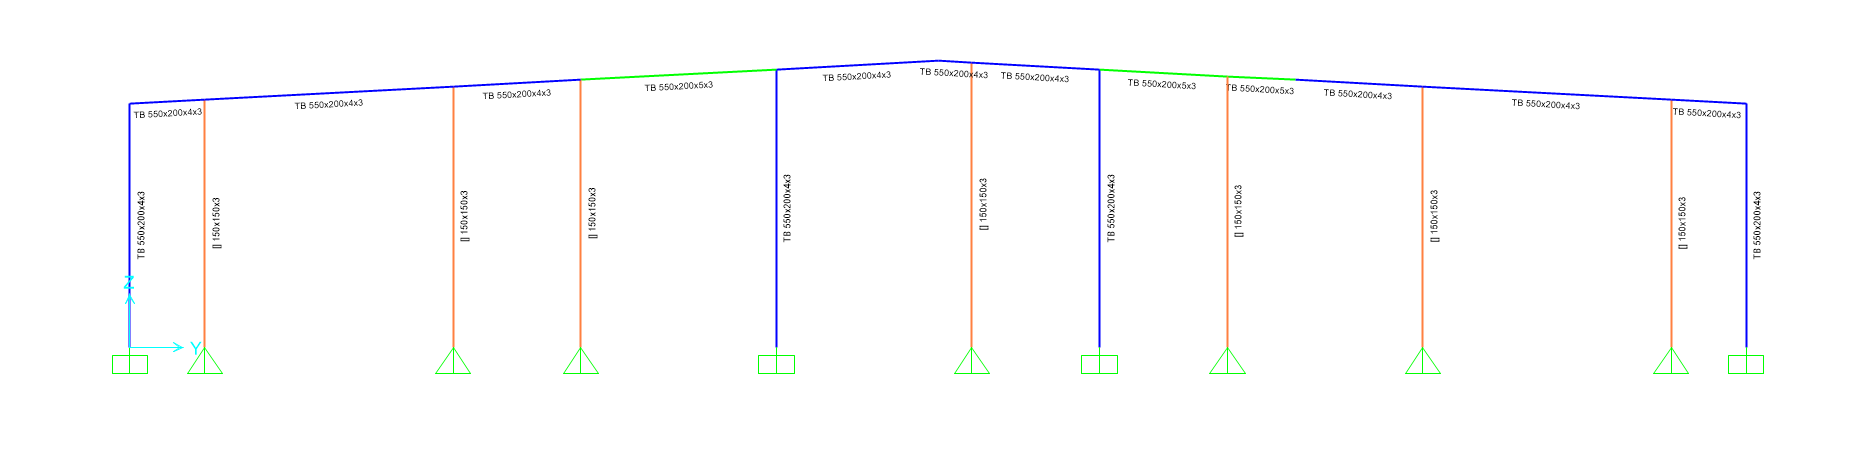
\includegraphics[width=\linewidth,height=2.2cm,keepaspectratio]{apoyos.png}\\[1mm]
  {\tiny Figura 11: Apoyos en la base --- empotrado [$\square$] en P1, articulado
   [$\triangle$] en P2 [SAP2000, elaboración propia].}
\end{center}
\end{frame}


%==================================================================
\section{Modelo SAP2000}
%==================================================================

%------------------------------------------------------------------
% 14. MODELO ESTRUCTURAL EN SAP2000
%------------------------------------------------------------------
\begin{frame}
\ctitle{MODELO ESTRUCTURAL EN SAP2000}
\begin{columns}[T,totalwidth=\textwidth]
  \column{0.45\textwidth}
  \vspace{-1mm}
  \begin{itemize}\scriptsize\setlength{\itemsep}{0mm}
    \item Modelo 3D con elementos \alert{frame}
          [barras]: columnas, vigas, correas y
          arriostramientos; base empotrada en pilares principales [P1] y apoyo simple en pilares secundarios [P2].
    \item \alert{Dos modelos idénticos} en geometría,
          secciones y cargas gravitacionales;
          difieren solo en \alert{espectros de diseño sísmico y presiones de viento}.
    \item Análisis \alert{modal espectral};
          $\xi = 0{,}03$.
  \end{itemize}
  \vspace{0mm}
  {\scriptsize\textbf{Dos escenarios de carga} [misma geometría y
  secciones]:}
  \begin{itemize}\scriptsize\setlength{\itemsep}{0mm}
    \item \alert{Instalado}: NCh2369.Of2003 +
          NCh432.Of1971.
    \item \alert{Actualizado}: NCh2369:2025 +
          NCh432:2025.
  \end{itemize}
  \column{0.52\textwidth}
  \vfill
  \centering
  \includegraphics[width=\linewidth,height=\imghS,keepaspectratio]%
    {slide16_img6.png}\\[1mm]
  \figcap{12}{Modelo SAP2000 --- vista 3D}{Elaboración propia}\\[1mm]
  \includegraphics[width=\linewidth,height=\imghS,keepaspectratio]%
    {slide16_img7.png}\\[1mm]
  \figcap{13}{Elevación transversal del modelo}{Elaboración propia}
  \vfill
\end{columns}
\end{frame}

%==================================================================

\section{Participación de masa modal}
%==================================================================

%------------------------------------------------------------------
% 15. PARTICIPACIÓN DE MASA MODAL
%------------------------------------------------------------------
\begin{frame}
\ctitle{PARTICIPACIÓN DE MASA MODAL}
\centering\vspace{-12mm}
{\footnotesize\textbf{Participación de masa modal} [común]:}\\[2mm]
\fittab{\tablasize
\begin{tabular}{@{}lrrr@{}}
  \toprule
    Dir. & Modo & $T$ [s] & Masa [\%] \\
    \midrule
    X [UX] & 26 & 0,2788 & 67,45\,\text{\%} \\
    Y [UY] & 22 & 0,3507 & 50,60\,\text{\%} \\
    Z [UZ] & 97 & 0,0185 & 42,10\,\text{\%} \\
    \bottomrule
  \end{tabular}}\\[4mm]
  {\scriptsize $\sum$UX$=$99,97\,\text{\%}; $\sum$UY$=$100,00\,\text{\%}; $\sum$UZ$=$99,80\,\text{\%}.\\[2mm]
  Periodos cortos $\Rightarrow$ estructura \alert{rígida}.}
  \end{frame}


\section{Cargas de diseño}
%==================================================================

%------------------------------------------------------------------
% 16. CARGAS DE DISEÑO
%------------------------------------------------------------------
\begin{frame}
\ctitle{CARGAS DE DISEÑO}
\vspace{1mm}
\begin{center}
  \fittab{\tablasize
  \begin{tabular}{@{}llp{5.4cm}@{}}
    \toprule
    Acción & Valor & Observación \\
    \midrule
    \multicolumn{3}{@{}l}{\textbf{Cargas permanentes [D]}} \\
    Peso propio      & SAP2000               & $+10\,\text{\%}$ por conexiones y pernos \\
    Cubierta KR-8    & $5{,}85$ kg/m$^2$      & Recubrimiento de techo \\
    Costaneras Z     & \alert{[pendiente]} kg/m$^2$ & No modeladas; aplicadas como carga \\
    \midrule
    \multicolumn{3}{@{}l}{\textbf{Sobrecargas}} \\
    Sobrecarga techo [Lr] & \alert{$53$} kg/m$^2$ & Reducida desde $100$ kg/m$^2$ \\
    Nieve [S]             & \alert{$25$} kg/m$^2$ & NCh431 1977 \\
    \midrule
    \multicolumn{3}{@{}l}{\textbf{Acciones ambientales}} \\
    Viento [W] & Presión  & NCh432 [1971 / 2025] \\
    Sismo [E]  & Espectro & NCh2369 [2003 / 2025] \\
    \bottomrule
  \end{tabular}}\\[3mm]
  {\capsize Tabla 1: Cargas de diseño [memoria original].}
\end{center}
\end{frame}

%==================================================================

\section{Combinaciones de carga}
%==================================================================

%------------------------------------------------------------------
% 17. COMBINACIONES DE CARGA
%------------------------------------------------------------------
\begin{frame}
\ctitle{COMBINACIONES DE CARGA}
\vspace{1mm}
\begin{itemize}\small\setlength{\itemsep}{3mm}
  \item Verificación por el método de \alert{Tensiones Admisibles [ASD]}, conforme a la
        normativa chilena [NCh3171 y NCh427/1, basada en AISC~360].
  \item Según \alert{NCh3171.Of2010} y combinaciones sísmicas
        según NCh2369 [2003/2025].
  \item Patrones: PP, CM\_CUB, CM\_MURO, L, S,
        Lr, Wx, Wy, Ex, Ey, Ez.
  \item Combinaciones generadas en SAP2000: \alert{46}
        [Instalado] vs \alert{214} [Actualizado].
  \item El fuerte aumento en 2025 refleja la
        \alert{tridimensionalidad} [casos $E_{x\text{-}a}$, $E_{y\text{-}a}$ y
        componente vertical $E_z$].
\end{itemize}
\vspace{2mm}
{\scriptsize\textit{Nota: la evaluación se realiza con la \textmd{NCh3171.Of2010}
por ser la versión empleada en el diseño original de la estructura. Existe una versión
actualizada, la \textmd{NCh3171:2017}, oficializada en 2024.}}
\end{frame}

%==================================================================

%------------------------------------------------------------------
% 18. APLICACIÓN DE COMBINACIONES AL MODELO SAP2000
%------------------------------------------------------------------
\begin{frame}
\ctitle{APLICACIÓN DE COMBINACIONES AL MODELO SAP2000}
\begin{columns}[T,totalwidth=\textwidth]
  \column{0.48\textwidth}
  \vspace{-1mm}
  {\footnotesize\textbf{Patrones y Casos de Carga [SAP2000]:}}\\[2mm]
  \fittab{\tablasize
  \begin{tabular}{@{}lll@{}}
    \toprule
    Atributo & Instalado [Original] & Actualizado [2025] \\
    \midrule
    Patrones de carga & 11 & \textbf{15} {\scriptsize [Nuevos: Ex-a, Ey-a, W$\pm$]} \\
    Sismo [Resp. Spec.] & 3 [Ex, Ey, Ez] & \textbf{5} {\scriptsize [+ Espectro amplificado]} \\
    Viento [Static] & 2 [Wx, Wy] & \textbf{4} {\scriptsize [Presiones direccionales]} \\
    Total Casos & 13 & \textbf{17} \\
    \bottomrule
  \end{tabular}
  }\\[3mm]
  \begin{itemize}\scriptsize\setlength{\itemsep}{2mm}
    \item La inclusión del \alert{espectro amplificado} [$E_{x-a}$, $E_{y-a}$] y las orientaciones del viento [$W_{x\pm}$, $W_{y\pm}$] aumentan los casos básicos.
  \end{itemize}

  \column{0.50\textwidth}
  \vspace{-1mm}
  {\footnotesize\textbf{Combinaciones de Carga Generadas:}}\\[2mm]
  \fittab{\tablasize
  \begin{tabular}{@{}lrr@{}}
    \toprule
    Métrica & Instalado & Actualizado \\
    \midrule
    Total combinaciones & \textbf{46} & \textbf{214} \alert{[$\uparrow 365\,\text{\%}$]} \\
    \bottomrule
  \end{tabular}
  }\\[3mm]
  \begin{itemize}\scriptsize\setlength{\itemsep}{2mm}
    \item El gran salto a \textbf{214 combinaciones} se debe a:
    \begin{enumerate}\scriptsize
      \item Permutaciones con los nuevos casos de viento y sismo amplificado.
      \item Inclusión de las \alert{combinaciones amplificadas} [$0{,}7R_1$] requeridas por la NCh2369:2025.
      \item Alternancia de cargas [$L$, $L_r$, $S$].
    \end{enumerate}
    \item \alert{Impacto:} El esfuerzo computacional y el volumen de revisión estructural se incrementan drásticamente bajo los nuevos estándares.
  \end{itemize}
\end{columns}
\end{frame}

\section{Viento: NCh432.Of1971}
%==================================================================

%------------------------------------------------------------------
% 19. VIENTO — NCh432.Of1971
%------------------------------------------------------------------
\begin{frame}
\ctitle{VIENTO --- NCh432.Of1971}
\vspace{2mm}
\begin{itemize}\small\setlength{\itemsep}{4mm}
  \item Norma oficial [DS N°994/1971]; presión básica \alert{uniforme}, sin
        zonificación geográfica.
  \item $q = u^2/16$ [kgf/m$^2$]; variación en altura
        $p_x = p_h\,(x/h)^{2\alpha}$ [$\alpha = 0{,}28$ urbano].
  \item Cargas por \alert{coeficientes de forma} $C$ [Figura 9]: muro barlovento
        $+0{,}80$, sotavento $-0{,}40$, cubierta $1{,}2\sin\theta - 0{,}4$.
  \item Sitio Nave~F: $q = \alert{65{,}92}$~kgf/m$^2$ a nivel de hombro [$h=8{,}19$~m];
        \alert{$68{,}47$} en la altura del parapeto [valor de diseño más desfavorable].
\end{itemize}
\end{frame}

%------------------------------------------------------------------
% 19b. VIENTO Of.1971 --- Figura 14 [presión vs altura]
%------------------------------------------------------------------
\begin{frame}
\ctitle{VIENTO Of.1971 --- PRESIÓN vs ALTURA}
\vspace{2mm}
\begin{center}
  \includegraphics[width=0.9\textwidth,height=0.74\textheight,keepaspectratio]%
    {fig02.png}\\[2mm]
  \figcap{14}{Presión $q$ vs altura [campo abierto / ciudad]}{Elaboración propia}
\end{center}
\end{frame}

%------------------------------------------------------------------
% 19c. VIENTO Of.1971 --- Figura 15 [coeficientes de forma]
%------------------------------------------------------------------
\begin{frame}
\ctitle{VIENTO Of.1971 --- COEFICIENTES DE FORMA}
\vspace{2mm}
\begin{center}
  \includegraphics[width=0.9\textwidth,height=0.74\textheight,keepaspectratio]%
    {nch71_fig9.png}\\[2mm]
  \figcap{15}{Coeficientes de forma sobre cubiertas [Anexo Fig. 9, NCh432.Of1971]}{NCh432.Of1971}
\end{center}
\end{frame}

%==================================================================

\section{Viento: NCh432:2025}
%==================================================================

%------------------------------------------------------------------
% 20. VIENTO — NCh432:2025
%------------------------------------------------------------------
\begin{frame}
\ctitle{VIENTO --- NCh432:2025}
\vspace{2mm}
\begin{itemize}\small\setlength{\itemsep}{4mm}
  \item 3.\textsuperscript{a} edición [jun 2025], base \alert{ASCE/SEI 7-22};
        \alert{procedimiento direccional}.
  \item $q_z = 0{,}613\,K_z K_{zt} K_e\,V^2$. Sitio: \alert{Zona III-A}, $V = 34$~m/s;
        Exposición B; $h = 8{,}19$~m, $G = 0{,}85$ $\Rightarrow$ $q_h = \alert{51{,}00}$~kgf/m$^2$.
  \item \alert{Edificio cerrado} [$GC_{pi} = \pm 0{,}18$]; $C_p$ por superficie y
        \alert{zonificación de cubierta} [h/2, h, 2h, resto].
\end{itemize}
\end{frame}

%------------------------------------------------------------------
% 20b. VIENTO 2025 --- Figura 16 [presiones netas]
%------------------------------------------------------------------
\begin{frame}
\ctitle{VIENTO 2025 --- PRESIONES NETAS}
\vspace{2mm}
\begin{center}
  \includegraphics[width=0.95\textwidth,height=0.74\textheight,keepaspectratio]%
    {slide06_img4.png}\\[2mm]
  \figcap{16}{Presiones netas sobre la Nave~F [NCh432:2025]}{Elaboración propia}
\end{center}
\end{frame}

%------------------------------------------------------------------
% 20c. VIENTO 2025 --- Figura 17 [coeficientes Cp]
%------------------------------------------------------------------
\begin{frame}
\ctitle{VIENTO 2025 --- COEFICIENTES $C_p$}
\vspace{2mm}
\begin{center}
  \includegraphics[width=0.9\textwidth,height=0.74\textheight,keepaspectratio]%
    {nch25_fig4_1.png}\\[2mm]
  \figcap{17}{Coeficientes de presión externa $C_p$ [SPRFV, Fig. 4, NCh432:2025]}{NCh432:2025}
\end{center}
\end{frame}

%==================================================================
\section{Viento: zonificación y presiones}
%==================================================================

%------------------------------------------------------------------
% 21. VIENTO — PRESIONES DE DISEÑO NCh432.Of1971
%------------------------------------------------------------------
\begin{frame}
\ctitle{VIENTO --- PRESIONES DE DISEÑO NCh432.Of1971}
\vspace{-1mm}
\begin{center}{\footnotesize
Presión básica $q = \alert{65{,}92}$~kgf/m$^2$ [$h = 8{,}19$~m, exposición ciudad].
Presión neta $p = C\cdot q$, con $C$ el \alert{coeficiente de forma} [Anexo Fig.~9].}
\end{center}
\vspace{2mm}
\begin{columns}[T,totalwidth=\textwidth]
  \column{0.49\textwidth}
  \centering
  {\footnotesize\textbf{Viento $\perp$ cara corta [Wx]}}\\[1.5mm]
  \fittab{\tablasize
  \begin{tabular}{@{}lrr@{}}
    \toprule
    Superficie & $C$ & $p$ [kgf/m$^2$] \\
    \midrule
    Muro barlovento  & $+0{,}80$ & $+52{,}74$ \\
    Techo-barlovento & $-0{,}34$ & $-22{,}20$ \\
    Techo-sotavento  & $-0{,}40$ & $-26{,}37$ \\
    Muro sotavento   & $-0{,}40$ & $-26{,}37$ \\
    \bottomrule
  \end{tabular}}
  \column{0.49\textwidth}
  \centering
  {\footnotesize\textbf{Viento $\perp$ cara larga [Wy]}}\\[1.5mm]
  \fittab{\tablasize
  \begin{tabular}{@{}lrr@{}}
    \toprule
    Superficie & $C$ & $p$ [kgf/m$^2$] \\
    \midrule
    Muro barlovento  & $+0{,}80$ & $+52{,}74$ \\
    Techo-barlovento & $-0{,}40$ & $-26{,}37$ \\
    Sotavento        & $-0{,}40$ & $-26{,}37$ \\
    \bottomrule
  \end{tabular}}
\end{columns}
\vspace{3mm}
{\scriptsize\centering Cubierta: $1{,}2\sin\theta - 0{,}4$ con $\theta \approx 3{,}02^\circ \Rightarrow -0{,}34$ [barlovento]. Valores: $+$ presión, $-$ succión.\par}
\end{frame}

%------------------------------------------------------------------
% 22. VIENTO — PRESIONES DE DISEÑO NCh432:2025
%------------------------------------------------------------------
\begin{frame}
\ctitle{VIENTO --- PRESIONES DE DISEÑO NCh432:2025}
\vspace{-2mm}
\begin{center}
  {\scriptsize $p = q\,K_d\,G\,C_p - q_h\,K_d\,(GC_{pi})$ \quad [Ec.~4]}\\[1mm]
  {\scriptsize $q_z = q_h = 51{,}00$;\quad $K_d = 0{,}85$;\quad $G = 0{,}85$;\quad $GC_{pi} = \pm0{,}18$.}
\end{center}
\vspace{1mm}
\begin{columns}[T,totalwidth=\textwidth]
  \column{0.47\textwidth}
  \centering
  {\footnotesize\textbf{$\perp$ Cara corta [Wx]}}\\[1.5mm]
  \fittab{\tablasize
  \begin{tabular}{@{}lrrr@{}}
    \toprule
    Superficie & $C_p$ & $W_{x+}$ [kgf/m$^2$] & $W_{x-}$ [kgf/m$^2$] \\
    \midrule
    Muro barlovento & $0{,}80$  & $21{,}68$  & $37{,}28$ \\
    Muro sotavento  & $-0{,}36$ & $-21{,}07$ & $-5{,}46$ \\
    Muros laterales & $-0{,}70$ & $-33{,}60$ & $-17{,}99$ \\
    Techo 0 a $h/2$ & $-0{,}90$ & $-40{,}97$ & $-25{,}36$ \\
    Techo $h/2$ a $h$ & $-0{,}90$ & $-40{,}97$ & $-25{,}36$ \\
    Techo $h$ a $2h$ & $-0{,}50$ & $-26{,}23$ & $-10{,}62$ \\
    Techo $> 2h$    & $-0{,}30$ & $-18{,}86$ & $-3{,}25$ \\
    \bottomrule
  \end{tabular}}
  \hfill
  \column{0.47\textwidth}
  \centering
  {\footnotesize\textbf{$\perp$ Cara larga [Wy]}}\\[1.5mm]
  \fittab{\tablasize
  \begin{tabular}{@{}lrrr@{}}
    \toprule
    Superficie & $C_p$ & $W_{y+}$ [kgf/m$^2$] & $W_{y-}$ [kgf/m$^2$] \\
    \midrule
    Muro barlovento & $0{,}80$  & $21{,}68$  & $37{,}28$ \\
    Muro sotavento  & $-0{,}50$ & $-26{,}23$ & $-10{,}62$ \\
    Muros laterales & $-0{,}70$ & $-33{,}60$ & $-17{,}99$ \\
    Techo 0 a $h/2$ & $-0{,}90$ & $-40{,}97$ & $-25{,}36$ \\
    Techo $h/2$ a $h$ & $-0{,}90$ & $-40{,}97$ & $-25{,}36$ \\
    Techo $h$ a $2h$ & $-0{,}50$ & $-26{,}23$ & $-10{,}62$ \\
    Techo $> 2h$    & $-0{,}30$ & $-18{,}86$ & $-3{,}25$ \\
    \bottomrule
  \end{tabular}}
\end{columns}
\vspace{2mm}
{\scriptsize\centering $W_{x+},W_{y+}$: presión interna $+0{,}18$ [Caso A]\quad $W_{x-},W_{y-}$: presión interna $-0{,}18$ [Caso B]. Valores en kgf/m$^2$ [$+$ presión, $-$ succión].\par}
\end{frame}

%------------------------------------------------------------------
% 23. VIENTO — CARGAS POR MARCO Wx [NCh432:2025]
%------------------------------------------------------------------
\begin{frame}
\ctitle{VIENTO --- CARGAS POR MARCO [NCh432:2025]}
\vspace{2mm}
\begin{center}
  \includegraphics[width=\linewidth,height=5.0cm,keepaspectratio]%
    {wind_Wx.png}\\[1.5mm]
  \figcap{18}{Cargas puntuales por marco --- viento $\perp$ cara corta [$W_x$]; zonas Z1--Z4 según $h$}{Elaboración propia}
\end{center}
\end{frame}

%------------------------------------------------------------------
% 24. VIENTO — CARGAS POR MARCO Wy [NCh432:2025]
%------------------------------------------------------------------
\begin{frame}
\ctitle{VIENTO --- CARGAS POR MARCO [NCh432:2025]}
\vspace{2mm}
\begin{center}
  \includegraphics[width=\linewidth,height=5.0cm,keepaspectratio]%
    {wind_Wy.png}\\[1.5mm]
  \figcap{19}{Cargas distribuidas por marco --- viento $\perp$ cara larga [$W_y$]; zonas NCh432:2025}{Elaboración propia}
\end{center}
\end{frame}

%------------------------------------------------------------------
% 25. VIENTO — ZONIFICACIÓN [gráfico]
%------------------------------------------------------------------
\begin{frame}
\ctitlesub{VIENTO — ZONIFICACIÓN Y PRESIONES}{Zonificación NCh432:2025}
\begin{center}
  \vspace{-2mm}
  \begin{tikzpicture}
    \node[anchor=south west,inner sep=0] (qzimg) at (0,0)
      {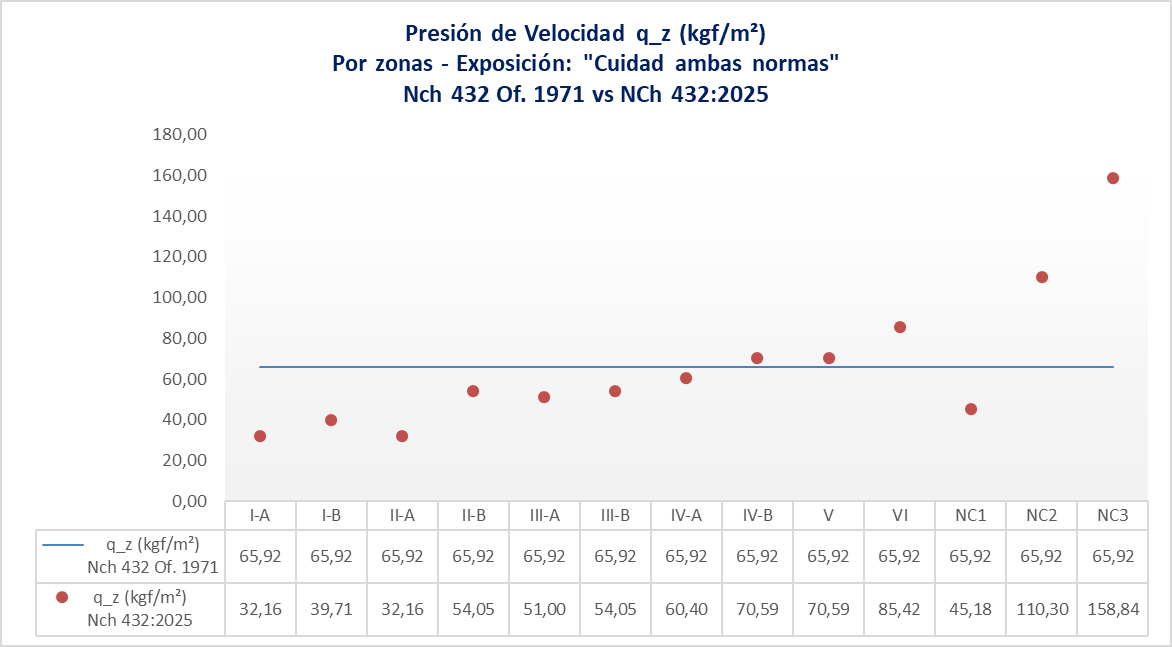
\includegraphics[width=0.68\linewidth,keepaspectratio]{fig_qz_zonas.png}};
    \begin{scope}[x={(qzimg.south east)},y={(qzimg.north west)}]
      \draw[red,very thick] (0.455,0.405) ellipse [x radius=0.022,y radius=0.05];
      \draw[red,very thick,->] (0.30,0.68) to[bend left=12] (0.44,0.45);
      \node[red,font=\scriptsize\bfseries,anchor=south east] at (0.31,0.685){Zona III-A};
    \end{scope}
  \end{tikzpicture}\\[2mm]
  \figcap{20}{$q_z$ por zona --- 1971 [uniforme, $65{,}92$\,kgf/m$^2$] vs 2025 [zonificada]. En Zona III-A: \alert{$51{,}00$\,kgf/m$^2$} [$-23\,\%$]}{Elaboración propia}
\end{center}
\end{frame}

%------------------------------------------------------------------
% 26. VIENTO — PRESIONES COMPARATIVAS [tablas]
%------------------------------------------------------------------
\begin{frame}
\ctitlesub{VIENTO — ZONIFICACIÓN Y PRESIONES}{Presiones comparativas 1971 vs 2025}
\begin{center}
{\small\textbf{Presión neta en muros} [kgf/m$^2$]:}\\[1mm]
\fittab{\tablasize
\begin{tabular}{@{}p{3cm}rrr@{}}
  \toprule
  Superficie & 1971 [kgf/m$^2$] & 2025 [kgf/m$^2$] & $\Delta$ \\
  \midrule
  Muro barlovento & $+52{,}74$ & $+37{,}28$ & $\downarrow 29\,\text{\%}$ \\
  Muro sotavento  & $-26{,}37$ & $-21{,}07$ & $\downarrow 20\,\text{\%}$ \\
  Muros laterales & ---        & $-33{,}60$ & nuevo \\
  \bottomrule
\end{tabular}}\\[2mm]
{\small\textbf{Succión en cubierta por zona} [$R = 2025/1971$]:}\\[1mm]
\fittab{\tablasize
\begin{tabular}{@{}p{3cm}rrr@{}}
  \toprule
  Zona & 1971 [kgf/m$^2$] & 2025 [kgf/m$^2$] & $\Delta\,\text{\%}$ \\
  \midrule
  0 a $h/2$    & $-26{,}37$ & $-40{,}97$ & $\uparrow 55\,\text{\%}$ \\
  $h/2$ a $h$  & $-26{,}37$ & $-40{,}97$ & $\uparrow 55\,\text{\%}$ \\
  $h$ a $2h$   & $-26{,}37$ & $-26{,}23$ & $\downarrow 1\,\text{\%}$ \\
  $> 2h$       & $-26{,}37$ & $-18{,}86$ & $\downarrow 28\,\text{\%}$ \\
  \bottomrule
\end{tabular}}\\[1.5mm]
{\small La 2025 \alert{intensifica} la succión de borde y \alert{alivia} la zona central.}
\end{center}
\end{frame}


%==================================================================
\section{Viento: solicitaciones globales}
%==================================================================

%------------------------------------------------------------------
% 27. VIENTO — PARÁMETROS DE DISEÑO
%------------------------------------------------------------------
\begin{frame}
\ctitlesub{VIENTO — SOLICITACIONES GLOBALES}{Parámetros de diseño}
\begin{columns}[T,totalwidth=\textwidth]
  \column{1.0\textwidth}
  \begin{center}
  {\footnotesize\textbf{Parámetros de Diseño de Viento [NCh432]:}}\\[2mm]
  \fittab{\tablasize
  \begin{tabular}{@{}lll@{}}
    \toprule
    Parámetro & Of.1971 & 2025 \\
    \midrule
    \textbf{Presión básica $q$} & \textbf{68,47 kgf/m$^2$} & \textbf{51,00 kgf/m$^2$} \alert{[$\downarrow 26\,\text{\%}$]} \\
    Exposición & Ciudad & Ciudad [Cat. B] \\
    Zona & --- & Zona III-A [$V=34$\,m/s] \\
    Categoría & --- & II [$I=1{,}00$] \\
    Tipo de techo & 2 Aguas & 2 Aguas [sim.] \\
    Cerramiento & --- & Cerrado [$GC_{pi} = \pm 0{,}18$] \\
    Efecto Venturi & No & --- \\
    Factor direccional $K_d$ & --- & 0,85 \\
    Factor topográfico $K_{zt}$ & --- & 1,0 \\
    Factor exposición $K_z$ & --- & $2{,}01(z/z_g)^{2/\alpha}$ \\
    Factor elevación $K_e$ & --- & 1,0 \\
    Factor ráfaga $G$ & --- & 0,85 \\
    \bottomrule
  \end{tabular}
  }\end{center}\vspace{1mm}
  \begin{itemize}\tiny\setlength{\itemsep}{1mm}
    \item La nueva normativa incorpora factores direccionales [$K_d$], topográficos [$K_{zt}$], exposición [$K_z$], elevación [$K_e$] y ráfaga [$G$], reduciendo la presión básica.
  \end{itemize}
\end{columns}
\end{frame}

%------------------------------------------------------------------
% 28. VIENTO — SOLICITACIONES GLOBALES
%------------------------------------------------------------------
\begin{frame}
\ctitlesub{VIENTO — SOLICITACIONES GLOBALES}{Evaluación por caso de carga}
\begin{columns}[T,totalwidth=\textwidth]
  \column{1.0\textwidth}
  \begin{center}
  {\footnotesize\textbf{Solicitaciones globales por caso de viento [tonf]:}}\\[2mm]
  \fittab{\tablasize
  \begin{tabular}{@{}lrrr@{}}
    \toprule
    Caso & Corte X [$F_x$] [tonf] & Corte Y [$F_y$] [tonf] & Levant. [$F_z$] [tonf] \\
    \midrule
    Wx [NCh432.Of1971] & 41,49 & 0 & 114,34 \\
    Wy [NCh432.Of1971] & 0 & 64,00 & 103,17 \\
    \midrule
    Wx+ [NCh432:2025] & 21,59 & 0 & 93,63 \\
    Wx- [NCh432:2025] & 21,58 & 0 & 28,46 \\
    Wy+ [NCh432:2025] & 0 & 33,51 & 93,58 \\
    Wy- [NCh432:2025] & 0 & 33,50 & 28,43 \\
    \bottomrule
  \end{tabular}
  }\end{center}\vspace{2mm}
  \begin{itemize}\scriptsize\setlength{\itemsep}{2mm}
    \item Cortes horizontales \alert{amplificados por parapeto} [factor $f = H_{\text{real}}/h_{\text{pilar}}$]; valores del modelo SAP2000.
    \item La norma 2025 introduce 4 casos direccionales [$W_{x\pm}$, $W_{y\pm}$] versus 2 casos de la norma 1971 [$W_x$, $W_y$].
  \end{itemize}
\end{columns}
\end{frame}

%==================================================================
\section{Sismo: NCh2369.Of2003}
%==================================================================

%------------------------------------------------------------------
% 28. SISMO — NCh2369.Of2003
%------------------------------------------------------------------
\begin{frame}
\ctitle{SISMO --- NCh2369.Of2003}
\begin{columns}[T,totalwidth=\textwidth]
  \column{0.50\textwidth}
  \vspace{-1mm}
  {\footnotesize\textbf{Parámetros de entrada --- Nave~F:}}\\[1mm]
  \fittab{\tablasize
  \begin{tabular}{@{}lll@{}}
    \toprule
    Parámetro & Valor & Ref. \\
    \midrule
    Zona / $A_0$    & 2 --- $0{,}30\,g$        & T.\,5.1/5.2 \\
    Suelo fundación & III --- Intermedio       & T.\,5.3/5.4 \\
                    & {\scriptsize $T'=0{,}62$\,s; $n=1{,}80$} & \\
    Importancia $I$ & $1{,}00$ [C2 Normal]     & Cl.\,4.3 \\
    Sistema $R$     & 4                        & T.\,5.6 \\
                    & {\scriptsize edif. ind. 1p, arr. discont.} & \\
    Amortig. $\xi$  & $0{,}03$                 & T.\,5.5 \\
    $C_{\text{máx}}$ & \alert{$0{,}203$}       & T.\,5.7 \\
    \bottomrule
  \end{tabular}}\\[2mm]
  {\scriptsize Análisis modal espectral [Ec.\,5-5]. La acción sísmica se evalúa de
  forma \alert{independiente en cada dirección horizontal} [$\pm E_x$, $\pm E_y$],
  combinada con la componente vertical [$\pm E_z$] según Cl. 5.1.1 y 5.5.}
  \column{0.48\textwidth}
  \vfill
  \centering
  \includegraphics[width=\linewidth,height=\imghM,keepaspectratio]%
    {espectro_2003_H.png}\\[1mm]
  \figcap{21}{Espectro horizontal de diseño NCh2369.Of2003; tope $C_{\text{máx}}=0{,}203\,g$ [Tabla 5.7]}{Elaboración propia}
  \vfill
\end{columns}
\end{frame}

%------------------------------------------------------------------
% 28b. SISMO — ACCIÓN SÍSMICA VERTICAL [Cl. 5.5.2]
%------------------------------------------------------------------
\begin{frame}
\ctitle{SISMO --- ACCIÓN SÍSMICA VERTICAL [Cl. 5.5.2]}
\begin{columns}[T,totalwidth=\textwidth]
  \column{0.48\textwidth}
  \vspace{-1mm}
  \begin{itemize}\footnotesize\setlength{\itemsep}{2.5mm}
    \item NCh2369.Of2003 \alert{Cl. 5.5.2}: alternativamente al método estático,
          se permite un \alert{análisis dinámico vertical} con el espectro de
          diseño [Ec. 5-5].
    \item Parámetros prescritos: \alert{$R=3$} y \alert{$\xi=0{,}03$}.
    \item La ordenada espectral \alert{no necesita superar $I\cdot A_0 = 0{,}30\,g$}.
  \end{itemize}
  \vspace{2mm}
  {\footnotesize\textbf{Espectro de diseño [Ec. 5-5]:}}\\[2mm]
  \centering
  {\small $S_a = \dfrac{2{,}75\,A_0\,I}{R}\left(\dfrac{T'}{T}\right)^{n}
  \left(\dfrac{0{,}05}{\xi}\right)^{0{,}4}$}
  \column{0.52\textwidth}
  \vfill
  \centering
  \includegraphics[width=\linewidth,height=\imghM,keepaspectratio]%
    {espectro_2003_V.png}\\[1mm]
  \figcap{22}{Espectro vertical NCh2369.Of2003 [Cl. 5.5.2; $R=3$, $\xi=0{,}03$]}{Elaboración propia}
  \vfill
\end{columns}
\end{frame}

%==================================================================

\section{Sismo: NCh2369:2025}
%==================================================================

%------------------------------------------------------------------
% 29. SISMO — NCh2369:2025
%------------------------------------------------------------------
\begin{frame}
\ctitle{SISMO --- NCh2369:2025}
\begin{columns}[T,totalwidth=\textwidth]
  \column{0.45\textwidth}
  \vspace{-1mm}
  \begin{itemize}\scriptsize\setlength{\itemsep}{0mm}
    \item Oficializada por \alert{Decreto Exento N°12}
          [MINVU]; vigencia obligatoria
          9-sep-2026.
    \item \alert{Nueva clasificación de suelos} [6 tipos,
          $V_{s30}$].
    \item El \alert{espectro de referencia} [Ec. 3, elástico] es la \alert{base}: el de
          \alert{diseño} $=I\,S_{aH}/R^{*}$ [acotado $C_{\text{mín}}$--$C_{\text{máx}}$]
          y el \alert{amplificado} $=0{,}7R_1\cdot$diseño.
    \item Combinaciones con \alert{amplificación sísmica}
          [casos $E_{x\text{-}a}$, $E_{y\text{-}a}$] y componente $E_z$.
  \end{itemize}
  \vspace{1mm}
  \begin{center}
  \fittab{\tablasize
  \begin{tabular}{@{}ll@{}}
    \toprule
    \multicolumn{2}{@{}l}{\textbf{Parámetros --- Nave~F [modelo]}} \\
    \midrule
    Zona / $A_0$ & 2 / 0,30g \\
    Tipo de suelo & C [homologación] \\
    $R$ / $R_v$  & 4 / 2 \\
    Periodos $T^*$ & $T^*_x = 0{,}2788$; $T^*_y = 0{,}3507$~s \\
    \bottomrule
  \end{tabular}}
  \end{center}
  \column{0.52\textwidth}
  \vfill
  \centering
  \includegraphics[width=\linewidth,height=\imghM,keepaspectratio]%
    {espectro_2025_H.png}\\[1mm]
  \figcap{23}{Espectro horizontal NCh2369:2025: \alert{referencia} [Ec. 3, elástico] $\to$ diseño [$C_{\text{máx}}=0{,}298$, $C_{\text{mín}}=0{,}110$] $\to$ amplificado [$0{,}7R_1$, $C_{\text{máx,amp}}=0{,}834$]}{Elaboración propia}
  \vfill
\end{columns}
\end{frame}

%------------------------------------------------------------------
% 29a2. SISMO — CLASIFICACIÓN DE SUELOS 2003 vs 2025
%------------------------------------------------------------------
\begin{frame}
\ctitle{SISMO --- CLASIFICACIÓN DE SUELOS [2003 vs 2025]}
\begin{columns}[T,totalwidth=\textwidth]
  \column{0.52\textwidth}
  \vspace{-1mm}
  \begin{itemize}\scriptsize\setlength{\itemsep}{2mm}
    \item \alert{Of.2003} [Tabla 4]: 4 tipos [I--IV] por descripción \alert{cualitativa}
          [roca, rígido, intermedio, blando]; parámetros $T'$ y $n$.
    \item \alert{2025} [Tablas 4 y 6]: 6 tipos [A--F] definidos por \alert{$V_{s30}$}
          [criterio cuantitativo]; más parámetros espectrales.
    \item Nave~F: el Suelo \alert{III} [2003] se \alert{homologa} a Suelo \alert{C}
          [2025] --- suelo denso o firme, $V_{s30}\ge 350$~m/s.
    \item El espectro 2025 usa más parámetros del suelo $\Rightarrow$ forma espectral
          más detallada [meseta, decaimiento y piso].
  \end{itemize}
  \vspace{1mm}
  {\scriptsize\textbf{Comparación:}}\\[1mm]
  \fittab{\tablasize
  \begin{tabular}{@{}lll@{}}
    \toprule
    Aspecto & Of.2003 & 2025 \\
    \midrule
    Criterio    & Cualitativo & $V_{s30}$ [m/s] \\
    N.\textsuperscript{o} tipos & 4 [I--IV] & 6 [A--F] \\
    Parámetros  & $T'$, $n$ & $S, r, T_0, p, q$ \\
    \bottomrule
  \end{tabular}}
  \column{0.46\textwidth}
  \vspace{-1mm}
  \centering
  {\scriptsize\textbf{Parámetros del suelo --- Tabla 6 [Suelo C]:}}\\[2mm]
  \fittab{\tablasize
  \begin{tabular}{@{}lc@{}}
    \toprule
    Parámetro & Suelo C \\
    \midrule
    $S$   & 1,05 \\
    $r$   & 4,50 \\
    $T_0$ & 0,40 s \\
    $p$   & 1,50 \\
    $q$   & 3,00 \\
    $T_1$ & 0,35 s \\
    \bottomrule
  \end{tabular}}\\[2mm]
  {\scriptsize Estos valores definen el espectro de referencia
  $S_{aH}=A_r S\,\dfrac{1+r(T/T_0)^p}{1+(T/T_0)^q}$ [Ec. 3].}
\end{columns}
\end{frame}

%------------------------------------------------------------------
% 29b. SISMO 2025 — ESPECTRO VERTICAL [R_V]
%------------------------------------------------------------------
\begin{frame}
\ctitle{SISMO 2025 --- ESPECTRO VERTICAL [$R_V$]}
\begin{columns}[T,totalwidth=\textwidth]
  \column{0.50\textwidth}
  \vspace{-1mm}
  \begin{itemize}\scriptsize\setlength{\itemsep}{2mm}
    \item \alert{$R_V$}: factor de modificación de respuesta para la dirección
          vertical [Tabla 7], \alert{independiente} del $R$ horizontal. No se calcula
          con $R^*$; se usa directo como divisor en la Ec. (2).
    \item \alert{$R_V = 2{,}0$} por defecto, salvo que se justifique por métodos
          reconocidos la validez de un valor mayor.
    \item El método estándar para la acción vertical es \alert{estático}
          [Cl. 5.7.1: $F_V = \pm C_V\,P$]; el espectro dinámico Ec. (2) aplica cuando
          la flexibilidad vertical sugiere deformaciones relevantes [Cl. 5.7.2].
  \end{itemize}
  \vspace{2mm}
  {\footnotesize\textbf{Espectro vertical de diseño [Ec. 2]:}}\\[2mm]
  \centering
  {\small $S_{a,v}(T_V) = \dfrac{I\,S_{aV}(T_V)}{R_V}
  \left(\dfrac{0{,}05}{\xi_V}\right)^{0{,}4}$}
  \column{0.50\textwidth}
  \vfill
  \centering
  \includegraphics[width=\linewidth,height=\imghM,keepaspectratio]%
    {espectro_2025_V.png}\\[1mm]
  \figcap{24}{Espectro vertical de diseño NCh2369:2025 [Ec. 2; $R_V=2$, $\xi_V=0{,}03$]}{Elaboración propia}
  \vfill
\end{columns}
\end{frame}

%==================================================================
\section{Resultados: Sismo — Comparativa de espectros}
%==================================================================

%------------------------------------------------------------------
% 30. SISMO — COMPARACIÓN DE ESPECTROS
%------------------------------------------------------------------
\begin{frame}
\ctitlesub{SISMO — COMPARATIVA DE ESPECTROS}{Of.2003 vs 2025}
\begin{columns}[T,totalwidth=\textwidth]
  \column{0.45\textwidth}
  \vspace{-1mm}
  {\footnotesize\textbf{Parámetros de Diseño Sísmico [NCh2369]:}}\\[2mm]
  \fittab{\tablasize
  \begin{tabular}{@{}lll@{}}
    \toprule
    Parámetro & Of.2003 & 2025 \\
    \midrule
    Zona [$A_0$] & 2 [$0{,}30g$] & 2 [$0{,}30g$] \\
    Suelo & III [Intermedio] & C [denso/firme] \\
    Importancia $I$ & 1,00 [Normal] & 1,00 \\
    Sistema $R$ & $R=4$ & $R=4$; $R_v=2$ \\
    Amortiguam. $\xi$ & 0,03 & 0,03 \\
    Períodos $T^*$ & \multicolumn{2}{c}{$T_x^*=0{,}2788$\,s;\ $T_y^*=0{,}3507$\,s\ \ [iguales, mismo modelo]} \\
    \bottomrule
  \end{tabular}}\\[4mm]
  \begin{itemize}\scriptsize\setlength{\itemsep}{2mm}
    \item Para la Nave F [$T \approx 0{,}28$--$0{,}35$\,s], el nuevo espectro es notablemente más restrictivo.
    \item Las combinaciones amplificadas [$0{,}7R_1$] incrementan sustancialmente las fuerzas de diseño en la nueva normativa.
  \end{itemize}
  
  \column{0.53\textwidth}
  \vfill
  \centering
  \includegraphics[width=\linewidth,keepaspectratio]%
    {espectros_comp.png}\\[1mm]
  \figcap{25}{Espectros NCh2369 Of.2003 vs 2025 generados a partir de los datos SAP2000}{Elaboración propia}
  \vfill
\end{columns}
\end{frame}


%==================================================================
\section{Resultados: Sismo — Reacciones en la Base}
%==================================================================

%------------------------------------------------------------------
% 31. SISMO — REACCIONES EN LA BASE
%------------------------------------------------------------------
\begin{frame}
\ctitlesub{SISMO — REACCIONES EN LA BASE}{Cortes basales y levantamiento}
\vspace{-1mm}
{\footnotesize\textbf{Comparativa de Corte Basal y Levantamiento [tonf]:}}\\[2mm]
\begin{center}
\fittab{\tablasize
\begin{tabular}{@{}lrrr|rrr|rrr@{}}
  \toprule
  & \multicolumn{3}{c}{\textbf{Instalado [1971]}} & \multicolumn{3}{c}{\textbf{Actualizado [2025]}} & \multicolumn{3}{c}{\textbf{Variación [$\Delta\,\text{\%}$]}} \\
  \cmidrule{2-4} \cmidrule{5-7} \cmidrule{8-10}
  Caso & $F_x$ & $F_y$ & $F_z$ & $F_x$ & $F_y$ & $F_z$ & $\Delta F_x$ & $\Delta F_y$ & $\Delta F_z$ \\
  \midrule
  $E_x$  & 11,52 & ---   & ---   & 16,75 & ---   & ---   & \textcolor{red}{$+45\,\text{\%}$} & --- & --- \\
  $E_y$  & ---   & 15,06 & ---   & ---   & 22,30 & ---   & --- & \textcolor{red}{$+48\,\text{\%}$} & --- \\
  $E_z$  & ---   & ---   & 10,22 & ---   & ---   & 11,50 & --- & --- & \textcolor{red}{$+13\,\text{\%}$} \\
  \midrule
  $E_{x-a}$ & ---   & ---   & ---   & \textbf{46,64} & ---   & ---   & \multicolumn{3}{c}{\multirow{2}{*}{\color{red} \textbf{Casos Amplificados}}} \\
  $E_{y-a}$ & ---   & ---   & ---   & ---   & \textbf{62,43} & ---   & \multicolumn{3}{c}{} \\
  \bottomrule
\end{tabular}
}
\end{center}\vspace{3mm}
\begin{itemize}\scriptsize\setlength{\itemsep}{2mm}
  \item Los espectros de diseño 2025 aumentan el corte basal estricto [$E_x, E_y$] en un ${\sim}45{-}48\,\text{\%}$.
  \item La inclusión de las componentes del \alert{espectro amplificado [$E_{x-a}, E_{y-a}$]} \alert{dispara} las reacciones a $46{-}62$\,tonf en combinación.
\end{itemize}
\end{frame}

%==================================================================
\section{Resultados: Desplazamientos}
%==================================================================

%------------------------------------------------------------------
% 33. SISMO — DESPLAZAMIENTOS
%------------------------------------------------------------------
\begin{frame}
\ctitlesub{RESULTADOS Y COMPARATIVAS}{Desplazamientos sísmicos — Nodo 76 [$h = 8{,}85$\,m]}
\vspace{1mm}
\begin{center}
\fittab{\tablasize
\begin{tabular}{@{}llrr>{\color{red}}r@{}}
  \toprule
  Dirección & Caso & Instalado [mm] & Actualizado [mm] & $\Delta\,\text{\%}$ \\
  \midrule
  \multirow{2}{*}{Sismo X [$U_1$]} & $E_x$ & 6,74 & \textbf{9,905} & $+47\,\text{\%}$ \\
                                   & $E_{x-a}$ & --- & \textbf{27,65} & --- \\
  \midrule
  \multirow{2}{*}{Sismo Y [$U_2$]} & $E_y$ & 5,62 & \textbf{8,258} & $+47\,\text{\%}$ \\
                                   & $E_{y-a}$ & --- & \textbf{81,17} & --- \\
  \midrule
  \multirow{2}{*}{Sismo Z [$U_3$]} & $E_z$ & 0,589 & \textbf{1,143} & $+94\,\text{\%}$ \\
                                   & $E_z$ amp. & --- & \textbf{---} & --- \\
  \bottomrule
\end{tabular}}
\end{center}\vspace{2mm}
\begin{itemize}\scriptsize\setlength{\itemsep}{2mm}
  \item Desplazamientos extraídos del nodo 76 [cumbrera, $h = 8{,}85$\,m]. Los casos $E_x$, $E_y$, $E_z$ corresponden al espectro estricto; $E_{x-a}$, $E_{y-a}$ al espectro amplificado [$0{,}7R_1$].
  \item El impacto del espectro amplificado genera un aumento drástico en las deformaciones sísmicas.
\end{itemize}
\end{frame}

%------------------------------------------------------------------
% 34. VIENTO — DESPLAZAMIENTOS
%------------------------------------------------------------------
\begin{frame}
\ctitlesub{RESULTADOS Y COMPARATIVAS}{Desplazamientos de viento — Nodo 76 [$h = 8{,}85$\,m]}
\vspace{1mm}
\begin{center}
\fittab{\tablasize
\begin{tabular}{@{}lllrrr@{}}
  \toprule
  Dirección & Caso Instalado & Caso Actualizado & Instalado [mm] & Actualizado [mm] & $\Delta\,\text{\%}$ \\
  \midrule
  Viento X [$U_1$] & $W_x$ & $W_{x+} / W_{x-}$ & 5,87 & 3,33 & {\color{verdeBox}$-43\,\text{\%}$} \\
  Viento Y [$U_2$] & $W_y$ & $W_{y+} / W_{y-}$ & 9,02 & 2,96 & {\color{verdeBox}$-67\,\text{\%}$} \\
  \bottomrule
\end{tabular}}
\end{center}\vspace{2mm}
\begin{itemize}\scriptsize\setlength{\itemsep}{2mm}
  \item Valores extraídos del nodo 76 [cumbrera, $h = 8{,}85$\,m]. Los desplazamientos por viento decrecen fuertemente con la nueva normativa [$W_{x\pm}$, $W_{y\pm}$].
  \item El \alert{sismo} se convierte en el caso que rige el control de deformaciones [$81{,}17\,$mm vs $2{,}96\,$mm en Y].
\end{itemize}
\end{frame}


%==================================================================
\section{Resultados: Factores de Utilización}
%==================================================================

%------------------------------------------------------------------
% 35. RESULTADOS Y COMPARATIVAS — FACTOR DE UTILIZACIÓN
%------------------------------------------------------------------
\begin{frame}
\ctitlesub{RESULTADOS Y COMPARATIVAS}{Factor de utilización máximo — Instalado vs Actualizado}
\vspace{-4mm}
\begin{center}
{\fontsize{7}{8.2}\selectfont
\fittab{
\setlength{\aboverulesep}{0.3mm}
\setlength{\belowrulesep}{0.3mm}
\renewcommand{\arraystretch}{0.85}
\begin{tabular}{@{}lllrcl@{}}
  \toprule
  Grupo & Perfil & Barra & F.U. & Estado & Combo \\
  \midrule
  \multicolumn{6}{@{}l}{\textbf{Instalado:}} \\
  \midrule
  Columnas 1 & TB $550\times200\times4\times3$ & 75  & 1,450 & \textcolor{red}{\textbf{NO CUMPLE}} & \texttt{\tiny D + Lr} \\
  Columnas 2 & {[}\,{]} $150\times150\times3$   & 318 & 2,162 & \textcolor{red}{\textbf{NO CUMPLE}} & \texttt{\tiny D + Wx} \\
  Columnas 3 & TBC $250\times150\times3$        & 192 & 0,234 & \textcolor{verdeBox}{\textbf{OK}}   & \texttt{\tiny D + Wx} \\
  Diagonal hor.  & {[}\,{]} $150\times150\times3$    & 16  & 0,830 & \textcolor{verdeBox}{\textbf{OK}}   & \texttt{\tiny D + Wx} \\
  Diagonales vert & {[}\,{]} $150\times150\times3$ & 283 & 0,779 & \textcolor{verdeBox}{\textbf{OK}}   & \texttt{\tiny D + Wx} \\
  Vigas 1        & TB $550\times200\times5\times3$   & 100 & 1,353 & \textcolor{red}{\textbf{NO CUMPLE}} & \texttt{\tiny D + Lr} \\
  Vigas 2        & {[}\,{]} $200\times200\times3$     & 160 & 0,146 & \textcolor{verdeBox}{\textbf{OK}}   & \texttt{\tiny D + Wx} \\
  \midrule
  \multicolumn{6}{@{}l}{\textbf{Actualizado [2025]:}} \\
  \midrule
  Columnas 1 \alert{*} & TB $550\times200\times4\times3$ & 103 & \textbf{1,474} & \textcolor{red}{\textbf{NO CUMPLE}} & \texttt{\tiny D+0.75$\cdot$((Ex-a+0.3Ey-a+0.3Ez)+Lr+L)} \\
  Columnas 2 \alert{*} & {[}\,{]} $150\times150\times3$   & 326 & \textbf{0,353} & \textcolor{verdeBox}{\textbf{OK}}   & \texttt{\tiny D+0.75$\cdot$((Ey-a+0.3Ex-a+0.3Ez)+Lr+L)} \\
  Columnas 3 \alert{*} & TBC $250\times150\times3$        & 191 & \textbf{0,794} & \textcolor{verdeBox}{\textbf{OK}}   & \texttt{\tiny D+Ex-a+0.3Ey-a+0.3Ez} \\
  Diagonal hor.  & {[}\,{]} $150\times150\times3$    & 181 & \textbf{0,737} & \textcolor{verdeBox}{\textbf{OK}}   & \texttt{\tiny D+0.75$\cdot$((Ex+0.3Ey+0.3Ez)+Lr+L)} \\
  Diagonales vert \alert{*} & {[}\,{]} $150\times150\times3$ & 294 & \textbf{2,265} & \textcolor{red}{\textbf{NO CUMPLE}} & \texttt{\tiny D+Ex-a+0.3Ey-a+0.3Ez} \\
  Vigas 1        & TB $550\times200\times5\times3$   & 109 & \textbf{1,173} & \textcolor{red}{\textbf{NO CUMPLE}} & \texttt{\tiny D+0.75$\cdot$((Ez+0.3Ex+0.3Ey)+Lr+L)} \\
  Vigas 2        & TBC $250\times150\times3$          & 404 & \textbf{0,125} & \textcolor{verdeBox}{\textbf{OK}}   & \texttt{\tiny D+Ey+0.3Ex+0.3Ez} \\
  \bottomrule
\end{tabular}}
}\end{center}
\vspace{1mm}
{\footnotesize \alert{*} Columnas y diagonales verticales: se consideró el sismo amplificado para el F.U.}
\end{frame}


%==================================================================
\section{Análisis comparativo}
%==================================================================

%------------------------------------------------------------------
% 36. ANÁLISIS COMPARATIVO — VARIACIÓN F.U.
%------------------------------------------------------------------
\begin{frame}
\ctitlesub{ANÁLISIS COMPARATIVO}{Variación de factores de utilización}
\vspace{2mm}
\begin{center}
\fittab{\tablasize
\begin{tabular}{@{}llrrr@{}}
  \toprule
  Grupo & Perfil & F.U. Instalado & F.U. Actualizado & $\Delta\,\text{\%}$ \\
  \midrule
  Columnas 1 \alert{*}  & TB $550\times200\times4\times3$ & 1,450 & \textbf{1,474} & \textcolor{red}{$+2\,\text{\%}$} \\
  Columnas 2 \alert{*}  & {[}\,{]} $150\times150\times3$   & 2,162 & \textbf{0,353} & \textcolor{verdeBox}{$-84\,\text{\%}$} \\
  Columnas 3 \alert{*}  & TBC $250\times150\times3$        & 0,234 & \textbf{0,794} & \textcolor{red}{$+239\,\text{\%}$} \\
  Diagonal hor.  & {[}\,{]} $150\times150\times3$    & 0,830 & \textbf{0,737} & \textcolor{verdeBox}{$-11\,\text{\%}$} \\
  Diagonales vert \alert{*} & {[}\,{]} $150\times150\times3$ & 0,779 & \textbf{2,265} & \textcolor{red}{$+191\,\text{\%}$} \\
  Vigas 1        & TB $550\times200\times5\times3$   & 1,353 & \textbf{1,173} & \textcolor{verdeBox}{$-13\,\text{\%}$} \\
  Vigas 2        & TBC $250\times150\times3$          & 0,089 & \textbf{0,125} & \textcolor{red}{$+40\,\text{\%}$} \\
  \bottomrule
\end{tabular}
}\end{center}\vspace{2mm}
\begin{itemize}\scriptsize\setlength{\itemsep}{1mm}
  \item Las \alert{diagonales verticales} presentan el mayor aumento [$+191\%$], alcanzando un F.U. crítico de $2{,}265$ con sismo amplificado.
  \item \alert{Columnas 2} [$-84\%$] y \alert{Diagonal hor.} [$-11\%$] mejoran sustancialmente su F.U. gracias a la combinación con $0{,}75R$.
  \item \alert{Vigas 1} se mantienen elevadas [F.U. $1{,}173$] pese a la reducción del $-13\%$.
\end{itemize}
{\footnotesize \alert{*} Columnas y diagonales verticales: se consideró el sismo amplificado para el F.U.}
\end{frame}

%------------------------------------------------------------------
% 37. ANÁLISIS COMPARATIVO — CORTES BASALES
%------------------------------------------------------------------
\begin{frame}
\ctitle{ANÁLISIS COMPARATIVO — CORTES BASALES}
\vspace{-2mm}
\begin{center}
\fittab{\tablasize
\begin{tabular}{@{}lrrr@{}}
  \toprule
  Indicador & Instalado [tonf] & Actualizado [tonf] & $\Delta$ \\
  \midrule
  \multicolumn{4}{@{}l}{\textbf{Viento [NCh432] — SAP2000:}} \\
  Corte basal X [$F_x$] & 41,49 & 21,59 & {\color{verdeBox}$\downarrow$48\%} \\
  Corte basal Y [$F_y$] & 64,00 & 33,51 & {\color{verdeBox}$\downarrow$48\%} \\
  Levantamiento Z [$F_z$, Wx] & 114,34 & 93,63 / 28,46 & {\color{verdeBox}$\downarrow$18\,/\,75\%} \\
  Levantamiento Z [$F_z$, Wy] & 103,17 & 93,58 / 28,43 & {\color{verdeBox}$\downarrow$9\,/\,72\%} \\
  \midrule
  \multicolumn{4}{@{}l}{\textbf{Sismo [NCh2369] — SAP2000:}} \\
  Corte basal X [$E_x$] & 11,52 & 16,75 & {\color{red}$\uparrow$45\%} \\
  Corte basal Y [$E_y$] & 15,06 & 22,30 & {\color{red}$\uparrow$48\%} \\
  Levantamiento Z [$E_z$] & 10,22 & 11,50 & {\color{red}$\uparrow$13\%} \\
  Corte basal X amplif. [$E_{x-a}$] & --- & 46,64 & --- \\
  Corte basal Y amplif. [$E_{y-a}$] & --- & 62,43 & --- \\
  \bottomrule
\end{tabular}}
\end{center}\vspace{1mm}
\begin{itemize}\tiny\setlength{\itemsep}{0.5mm}
  \item \alert{Viento}: demanda lateral \alert{disminuye} $\sim$48\% [con amplificación por parapeto]. Levantamiento varía según presión interna.
  \item \alert{Sismo}: demanda \alert{aumenta} [$+45$ a $+48\%$; amplificado hasta $62{,}43$\,tonf].
  \item \alert{Cambio de carga dominante}: de viento [Instalado] a \alert{sismo} [Actualizado].
  \item \alert{Elementos críticos}: diagonales y columnas superan \alert{F.U. $> 1{,}0$} $\Rightarrow$ requieren \alert{adecuación}.
\end{itemize}
\end{frame}

%==================================================================
\section{Idealización y costos}
%==================================================================

%------------------------------------------------------------------
% 37b. IDEALIZACIÓN DEL MODELO
%------------------------------------------------------------------
\begin{frame}
\ctitle{IDEALIZACIÓN DEL MODELO}
\begin{columns}[T,totalwidth=\textwidth]
  \column{0.49\textwidth}
  \vspace{-1mm}
  \begin{itemize}\scriptsize\setlength{\itemsep}{1.8mm}
    \item Modelo Actualizado: \alert{114 de 274} elementos [42\%] no cumplen
          [F.U. $>1{,}0$], concentrados en \alert{5 grupos}.
    \item Idealización: sustituir esos grupos por secciones mayores [catálogo \alert{TUBEST}
          y \alert{AISC W}], con el \alert{mínimo acero} y conservando la tipología.
    \item Causa raíz: el cajón $\square\,150\times150\times3$ [$A=17{,}6$~cm$^2$] quedó
          subdimensionado en diagonales y columnas; los cajones de vigas, cortos en flexión.
    \item En vigas, la flexión supera cualquier cajón $\Rightarrow$ se usa \alert{perfil W de
          ala ancha} [W\,$12\times72$] para que no gobierne el pandeo lateral-torsional.
    \item Resultado: \alert{0 de 274} exceden la unidad; razón máxima \alert{0,81} [Vigas 1]
          $\Rightarrow$ \textcolor{verdeBox}{\textbf{cumple}}.
  \end{itemize}
  \column{0.50\textwidth}
  \centering
  {\scriptsize\textbf{Sustitución de perfiles [Tabla 39]:}}\\[1.5mm]
  \fittab{\tablasize
  \begin{tabular}{@{}llc@{}}
    \toprule
    Grupo & Sección propuesta & D/C \\
    \midrule
    Diagonales vert. & TB $250\times225\times4\times3$ & $2{,}26\to0{,}52$ \\
    Diagonal horiz.  & TC $300\times150\times3$        & $1{,}46\to0{,}69$ \\
    Columnas 2       & TC $300\times150\times3$        & $1{,}92\to0{,}76$ \\
    Columnas 1       & W $12\times72$                  & $1{,}47\to0{,}79$ \\
    Vigas 1          & W $12\times72$                  & $1{,}35\to0{,}81$ \\
    \bottomrule
  \end{tabular}}\\[2mm]
  {\scriptsize Verificación 2-pass NCh2369:2025 [combinaciones amplificadas $0{,}7R_1$].
  Razón máx. final: \alert{0,81}.}
\end{columns}
\end{frame}

%------------------------------------------------------------------
% 37c. PESO ESTRUCTURAL Y COSTOS
%------------------------------------------------------------------
\begin{frame}
\ctitle{PESO ESTRUCTURAL Y COSTOS}
\begin{columns}[T,totalwidth=\textwidth]
  \column{0.50\textwidth}
  \vspace{-1mm}
  \begin{itemize}\scriptsize\setlength{\itemsep}{2.2mm}
    \item Como la configuración idealizada \alert{sí cumple}, se cuantifica su acero y costo.
          Solo cambian los \alert{5 grupos}; el resto se mantiene.
    \item Precio de referencia: \alert{1.400 CLP/kg} de acero instalado [CYPE Chile, 2025;
          rango $1.384$--$1.414$].
    \item El acero del sistema principal pasa de \alert{59.784} a \alert{116.185 kg}
          [\alert{+94\%}, prácticamente el doble].
    \item Costo estimado: \alert{83,7 $\to$ 162,7 millones CLP}; sobrecosto de material
          \alert{$\sim$79 millones}, concentrado en Vigas 1 y Columnas 1 [perfiles W\,$12\times72$].
    \item Adecuación \alert{viable} sin alterar la geometría, pero \alert{casi duplica} el
          acero. [Solo material; sin conexiones ni montaje.]
  \end{itemize}
  \column{0.48\textwidth}
  \centering
  {\scriptsize\textbf{Peso y costo total [Tabla 42]:}}\\[1.5mm]
  \fittab{\tablasize
  \begin{tabular}{@{}lrr@{}}
    \toprule
    Grupo & Peso act.$\to$ideal. [kg] & $\Delta$ costo \\
    \midrule
    Vigas 1          & 25.736 $\to$ 53.675 & +39,1 M \\
    Columnas 1       & 15.414 $\to$ 36.316 & +29,3 M \\
    Diagonal horiz.  & 9.096 $\to$ 14.317  & +7,3 M \\
    Diagonales vert. & 1.194 $\to$ 2.759   & +2,2 M \\
    Columnas 2       & 1.347 $\to$ 2.121   & +1,1 M \\
    Resto            & 6.997 $\to$ 6.997   & 0 \\
    \midrule
    \textbf{TOTAL}   & \textbf{59.784 $\to$ 116.185} & \textbf{+79,0 M} \\
    \bottomrule
  \end{tabular}}\\[1.5mm]
  {\scriptsize $\Delta$ costo en millones de CLP [$1.400$ CLP/kg].}
\end{columns}
\end{frame}

%------------------------------------------------------------------
% 38. CONCLUSIONES
%------------------------------------------------------------------
\begin{frame}
\ctitle{CONCLUSIONES}
\vspace{-2mm}
\begin{itemize}\scriptsize\setlength{\itemsep}{1.6mm}
  \item \alert{Viento [NCh432:2025]} --- \alert{reduce} la demanda: la presión de referencia
        baja $-26\%$ [$68{,}47 \to 51{,}00$\,kgf/m$^2$] y el corte basal cae $\sim$45\%
        [$W_x$: $41{,}5\to21{,}6$; $W_y$: $64{,}0\to33{,}5$\,tonf]. Pero zonifica la cubierta
        con \alert{succiones de borde mayores} $\Rightarrow$ exige verificar las fijaciones.
  \item \alert{Sismo [NCh2369:2025]} --- \alert{aumenta} la demanda: el corte basal crece
        $+45\%$ en X y $+47\%$ en Y, e incorpora las direcciones \alert{amplificadas}
        [$E_{x\text{-}a}=46{,}4$; $E_{y\text{-}a}=62{,}0$\,tonf], que pasan a \alert{gobernar}
        el diseño.
  \item \alert{Suficiencia del diseño original}: bajo el escenario Actualizado varios grupos
        del sistema resistente principal \alert{dejan de cumplir} [F.U. hasta $2{,}26$]. Es la
        actualización \alert{sísmica} --- no la de viento --- la que determina la intervención.
  \item \alert{Adecuación}: sustituyendo \alert{5 grupos} por secciones mayores [tubulares
        TUBEST en diagonales/columnas y \alert{perfiles W de ala ancha} en vigas y columnas
        principales] la estructura \alert{cumple} [0/274; razón máx $0{,}81$], sin alterar la
        geometría. Su costo no es menor: el acero pasa de $59.784$ a $116.185$~kg [\alert{+94\%}],
        con un sobrecosto de material $\sim$\alert{79 millones CLP}.
  \item \alert{Síntesis}: la Nave~F, satisfactoria bajo las normas con que fue concebida,
        \alert{no cumple} las exigencias de 2025 [principalmente por el incremento sísmico],
        pero su \alert{adecuación es viable} por redimensionamiento. La verificación completa
        [deflexiones, distorsiones, conexiones] es la continuación natural del trabajo.
\end{itemize}
\end{frame}

%==================================================================
% REFERENCIAS
%==================================================================

%------------------------------------------------------------------
% 39. REFERENCIAS — Normas Chilenas
%------------------------------------------------------------------
\begin{frame}
\ctitle{REFERENCIAS}
\vspace{-1mm}
\scriptsize\textbf{Normas Chilenas [INN]}\\[1mm]
\begin{itemize}\scriptsize\setlength{\itemsep}{0.5mm}
  \item Instituto Nacional de Normalización [1971]. \textit{NCh432 Of.1971:
        Acción del viento sobre las construcciones.} Santiago: INN.
  \item ——\,[2003]. \textit{NCh2369 Of.2003: Diseño sísmico de estructuras
        e instalaciones industriales.} Santiago: INN.
  \item ——\,[2010]. \textit{NCh3171.Of2010: Diseño estructural —
        Disposiciones básicas y combinaciones de carga.} Santiago: INN.
  \item ——\,[2019]. \textit{NCh427/2:2019: Diseño y construcción en acero
        — Parte 2: Estructuras con elementos conformados en frío.}
        Santiago: INN.
  \item ——\,[2025a]. \textit{NCh2369:2025: Diseño sísmico de estructuras
        e instalaciones industriales.} Santiago: INN.
  \item ——\,[2025b]. \textit{NCh432:2025: Diseño estructural — Cargas de
        viento.} Santiago: INN.
\end{itemize}
\end{frame}

%------------------------------------------------------------------
% 40. REFERENCIAS — Normas Internacionales y Libro de Texto
%------------------------------------------------------------------
\begin{frame}
\ctitle{REFERENCIAS}
\vspace{-1mm}
\scriptsize\textbf{Normas Internacionales y Libro de Texto}\\[1mm]
\begin{itemize}\scriptsize\setlength{\itemsep}{0.5mm}
  \item American Institute of Steel Construction [2022]. \textit{ANSI/AISC
        360-22: Specification for Structural Steel Buildings.}
        Chicago: AISC.
  \item American Iron and Steel Institute [2016]. \textit{AISI S100-16:
        North American Specification for the Design of Cold-Formed Steel
        Structural Members.} Washington: AISI.
  \item ——\,[2020]. \textit{AISI S100-16 with Supplement 3 [2020].}
        Washington: AISI.
  \item ASTM International [2019]. \textit{ASTM A36/A36M-19: Standard
        Specification for Carbon Structural Steel.}
        West Conshohocken: ASTM.
  \item Computers and Structures Inc. [2020]. \textit{CSI Analysis Reference
        Manual for SAP2000.} Berkeley: CSI.
  \item Pi Luco, J. [s.f.]. \textit{Diseño de Estructuras de Acero con
        Análisis y Aplicaciones basado en ANSI/AISC360 y AISI S100.}
        1.\textsuperscript{a}\,ed. Santiago.
\end{itemize}
\end{frame}

%==================================================================
% 41. CONTRAPORTADA
%------------------------------------------------------------------
\begin{frame}[plain]
  \vspace*{0.5cm}
  \titlepage
  \addplainfoot
\end{frame}

\end{document}
